% Modelo de TCC do Bacharelado em Ciência da Computação da UNIFESP 
% Baseado no Modelo de Documentos Academicos do ABNTex2  

\documentclass[	12pt, Times, openright, twoside, a4paper, english, brazil]{abntex2}

% ---
% Pacotes fundamentais 
% ---
\usepackage{cmap}				% Mapear caracteres especiais no PDF
%\usepackage{lmodern}			% Usa a fonte Latin Modern			
\usepackage{times}
\usepackage[T1]{fontenc}			% Selecao de codigos de fonte.
\usepackage[utf8]{inputenc}		% Codificacao do documento (conversão automática dos acentos)
\usepackage{lastpage}			% Usado pela Ficha catalográfica
%\usepackage{natbib}
\usepackage{indentfirst}			% Indenta o primeiro parágrafo de cada seção.
\usepackage{color}				% Controle das cores
\usepackage{graphicx, url}			% Inclusão de gráficos
\usepackage{hyperref}
\usepackage{xr}
\usepackage{color}
\usepackage{listings}
\newcommand{\todo}[1]{\textcolor{red}{@TODO: #1}}

\lstset{language=C, breaklines=true,
	inputencoding=utf8,
    extendedchars=true,
    literate={á}{{\'a}}1 {ã}{{\~a}}1 {é}{{\'e}}1
}
% ---

% ---
% Pacotes de citações
% ---
\usepackage[brazilian,hyperpageref]{backref}	 % Paginas com as citações na bibl
\usepackage[alf]{abntex2cite}	% Citações padrão ABNT

% --- 
% CONFIGURAÇÕES DE PACOTES
% --- 

% ---
% Configurações do pacote backref
% Usado sem a opção hyperpageref de backref
\renewcommand{\backrefpagesname}{Citado na(s) página(s):~}
% Texto padrão antes do número das páginas
\renewcommand{\backref}{}
% Define os textos da citação
\renewcommand*{\backrefalt}[4]{
	\ifcase #1 %
		Nenhuma citação no texto.%
	\or
		Citado na página #2.%
	\else
		Citado #1 vezes nas páginas #2.%
	\fi}%
% ---

% numeração de figuras e tabelas 
\counterwithout{figure}{section}
\counterwithout{table}{section}

%\renewcommand\tablename{Tabela{\arabic{chapter}.}}


% ---
% Informações de dados para CAPA e FOLHA DE ROSTO
% ---
\titulo{DESENVOLVIMENTO E SIMULAÇÃO DE SOFTWARE DE CONTROLE PARA UM PROTÓTIPO DE BOMBA DE INFUSÃO DE INSULINA BASEADOS EM MICROCONTROLADOR DA FAMÍLIA PIC}
\autor{Dinesh Atul Rodrigues Trivedi}
\local{São José dos Campos, SP}
\data{Julho de 2014}
\orientador{Prof. Dr. Luiz Eduardo Galvão Martins}
\instituicao{%
  Universidade Federal de São Paulo -- UNIFESP
  \par
  Instituto de Ciência de Tecnologia
  \par
  Bacharelado em Ciência da Computação}
\tipotrabalho{Trabalho de Graduação}
% O preambulo deve conter o tipo do trabalho, o objetivo, 
% o nome da instituição e a área de concentração 
\preambulo{Trabalho de conclusão de curso apresentado ao Instituto de Ciência e Tecnologia – UNIFESP, como parte das atividades para obtenção do título de Bacharel em Ciência da Computação.}
% ---

% informações do PDF
\makeatletter
\hypersetup{
     	%pagebackref=true,
		pdftitle={\@title}, 
		pdfauthor={\@author},
    	pdfsubject={\imprimirpreambulo},
	    pdfcreator={LaTeX with abnTeX2},
		pdfkeywords={abnt}{latex}{abntex}{abntex2}{trabalho acadêmico}, 
		colorlinks=true,       		% false: boxed links; true: colored links
    	linkcolor=blue,          	% color of internal links
    	citecolor=blue,        		% color of links to bibliography
    	filecolor=magenta,      		% color of file links
		urlcolor=blue,
		bookmarksdepth=4
}

\makeatother
% --- 
% --- 
% Espaçamentos entre linhas e parágrafos 
% --- 
% O tamanho do parágrafo é dado por:
\setlength{\parindent}{1.3cm}
% Controle do espaçamento entre um parágrafo e outro:
\setlength{\parskip}{0.2cm}  % tente também \onelineskip
% ---

% compila o indice
% ---
\makeindex
% ---

% ----
% Início do documento
% ----
\begin{document}
% Retira espaço extra obsoleto entre as frases.
\frenchspacing 

% ----------------------------------------------------------
% ELEMENTOS PRÉ-TEXTUAIS
% ----------------------------------------------------------
% \pretextual

% ---
% Capa
% ---
\begin{capa}
  \begin{center}
   
\includegraphics[width=.25\textwidth]{logo-unifesp.pdf}
    \vspace*{\fill}
    
    {\ABNTEXchapterfont\large\imprimirautor}
    \vspace*{\fill}
    
    {\ABNTEXchapterfont\bfseries\Large\imprimirtitulo}
    \vspace*{\fill}\vspace*{\fill}
    
   \imprimirlocal
   \end{center}
\end{capa}

% ---
% Folha de rosto
% (o * indica que haverá a ficha bibliográfica)
% ---
\imprimirfolhaderosto*
% ---

% ---
% Inserir folha de aprovação
% ---
% Isto é um exemplo de Folha de aprovação, elemento obrigatório da NBR
% 14724/2011 (seção 4.2.1.3). Você pode utilizar este modelo até a aprovação
% do trabalho. Após isso, substitua todo o conteúdo deste arquivo por uma
% imagem da página assinada pela banca com o comando abaixo:
%
% \includepdf{folhadeaprovacao_final.pdf}
%
\begin{folhadeaprovacao}
  \begin{center}
    {\ABNTEXchapterfont\large\imprimirautor}

    \vspace*{\fill}\vspace*{\fill}
    {\ABNTEXchapterfont\bfseries\Large\imprimirtitulo}
    \vspace*{\fill}
    
    \hspace{.45\textwidth}
    \begin{minipage}{.5\textwidth}
        \imprimirpreambulo
    \end{minipage}%
    \vspace*{\fill}
   \end{center}
    
   Trabalho aprovado em 01 de Julho de 2013:

   \assinatura{\textbf{\imprimirorientador} \\ Orientador} 
   \assinatura{\textbf{Prof. Dr. Tiago de Oliveira} \\ Convidado 1}
   \assinatura{\textbf{Prof. Dr. Fabiano C. Paixão} \\ Convidado 2}
%   \assinatura{\textbf{Professor} \\ Convidado 3}
   %\assinatura{\textbf{Professor} \\ Convidado 4}
      
   \begin{center}
    \vspace*{0.5cm}
    {\large\imprimirlocal}
    \par
    {\large\imprimirdata}
    \vspace*{1cm}
  \end{center}
  
\end{folhadeaprovacao}
% ---

% ---
% Dedicatória
% ---
\begin{dedicatoria}
   \vspace*{\fill}
   \centering
   \noindent
   \textit{ Este trabalho é dedicado  ... } \vspace*{\fill}
\end{dedicatoria}
% ---

% ---
% Agradecimentos
% ---
\begin{agradecimentos}
Escreva aqui os agradecimentos ...

\end{agradecimentos}
% ---

% ---
% Epígrafe
% ---
\begin{epigrafe}
    \vspace*{\fill}
	\begin{flushright}
		\textit{``Não vos amoldeis às estruturas deste mundo, \\
		mas transformai-vos pela renovação da mente, \\
		a fim de distinguir qual é a vontade de Deus: \\
		o que é bom, o que Lhe é agradável, o que é perfeito.\\
		(Bíblia Sagrada, Romanos 12, 2)}
	\end{flushright}
\end{epigrafe}
% ---

% ---
% RESUMOS
% ---

% resumo em português
\begin{resumo}
Estima-se que o Diabetes Melito (DM) já afeta 246 milhões de pessoas em todo mundo. A estimativa é que aumente para 380 milhões até 2025, sendo que no Brasil esse número chegue à aproximadamente 7 milhões. Seu tratamento adequado, na maioria das vezes, é o uso contínuo da bomba de infusão de insulina, entretanto é inacessível a grande parte da população, devido ao seu alto custo, aproximadamente R\$ 14.000,00. Sendo assim,este projeto tem como objetivo o desenvolvimento de um sistema embarcado crítico de controle de protótipo de bomba de infusão de insulina, baseado no microcontrolador da família PIC, PIC18F452. Neste trabalho utilizou-se o compilador MikroC que dá suporte aos periféricos necessários através de uma biblioteca completa em C. O desenvolvimento utilizou conceito de OOC, \emph{Object Orientated Programming in ANSI-C}, para desacoplamento de todos os módulos existentes. Esse conceito possibilitou o uso de \emph{Design Patterns}, ambos contribuíram para aumentar a capacidade de expandir e dar manutenção ao \emph{software} de forma mais simples. Os testes do software foram realizados através do simulador Proteus, o que possibilita uma grande facilidade para o depuramento. O circuito montado nesse simulador contém todos os componentes reais necessários para o desenvolvimento do protótipo. E,além disso, optou-se pelo uso do Proteus devido as grandes vantagens e minimização de problemas de integração que um simulador proporciona. Por fim esse projeto serve como uma prova de conceito para o problema abordado, demonstrando a evolução e problemas encontrados durante o desenvolvimento. Servindo como base para projetos futuros.

 
 \vspace{\onelineskip}
    
 \noindent
 \textbf{Palavras-chaves}: PIC, Microcontrolador, Sistema embarcado, Sistema crítico, Motor de passo, OOC.
\end{resumo}

% resumo em inglês
\begin{resumo}[Abstract]
\begin{otherlanguage*}{english}
It is estimated that diabetes mellitus (DM) already affects 246 million people around world. It is estimated to increase to 380 million by 2025, and in Brazil this the number will reach about 7 million. Adequate treatment in most times, is the continuous use of insulin pump therapy, however it is inaccessible to a large part of the population due to its high cost approximately R\$ 14,000.00. Thus, this project aims to develop an embedded system critical control prototype insulin infusion pump based microcontroller family PIC, PIC18F452. In this study we used the MikroC compiler that supports the required peripherals through a complete library in C. The development concept used OOC \ emph {Object Orientated Programming in ANSI-C} for decoupling of all the modules. This concept allowed the use of \ emph {Design Patterns}, both contributed to increase the ability to expand and maintain the \ emph {software} in a simpler way. The tests were performed using the software simulator Proteus, which allows a great facility for the depuration. The circuit used in simulator  contains all the components necessary for real prototype development. 
Also, Proteus was chosen because of the great benefits and minimize integration problems that a simulator provides. Finally this project serves as a proof of concept for the addressed problem, demonstrating the progress and problems encountered during development. Serving as a base for future projects.

   \vspace{\onelineskip}
 
   \noindent 
   \textbf{Key-words}: PIC, Microcontroler, Embedded System, Critical System, Step Motor, OOC.
\end{otherlanguage*}
\end{resumo}

% ---
% inserir lista de ilustrações
% ---
\pdfbookmark[0]{\listfigurename}{lof}
\listoffigures*
\cleardoublepage
% ---

% ---
% inserir lista de tabelas
% ---
\pdfbookmark[0]{\listtablename}{lot}
\listoftables*
\cleardoublepage
% ---

% ---
% inserir lista de abreviaturas e siglas
% ---
\begin{siglas}
  \item[$\mu$A] Microampére
  \item[ADC] \emph{Analogic Digital Conversor}
  \item[A/D] \emph{Analogic Digital}
  \item[CA] Corrente alternada
  \item[CC] Corrente contínua
  \item[CCP] \emph{Capture} / \emph{Compare} / \emph{PWM}
  \item[DM] Diabetes Melito
  \item[EEPROM] \emph{Electrically-Erasable Programmable Read-Only Memory}
  \item[I/O] Entrada/Saída
  \item[IDE] \emph{Integrated Development Environment}
  \item[kHzs] \emph{Kilohertz}
  \item[LCD] \emph{Liquid Crystal Display}
  \item[LVD] \emph{Low Voltage Detect}
  \item[mA] Miliampére
  \item[MCLR] \emph{Master Clear or Reset}
  \item[MHz] \emph{Megahertz}
  \item[MIPS] Milhões de Instruções por Segundo
  \item[MSSP] \emph{Master Synchronous Serial Port}
  \item[OO] Orientado à Objetos
  \item[OOC]  \emph{Object Orientated Programming in ANSI-C}
  \item[PC] \emph{Personal Computer}
  \item[PSP] \emph{Parallel Slave Port}
  \item[PWM] \emph{Pulse-Width Modulation}
  \item[RAM] \emph{Random Access Memory}          
  \item[ROM] \emph{Read-Only Memory}
  \item[TTL] \emph{Transistor-transistor Logic}
  \item[V] Volts  
\end{siglas}
% ---

% ---
% inserir lista de símbolos
% ---
\begin{simbolos}
  \item[$ \mu $] micro
\end{simbolos}
% ---

% ---
% inserir o sumario
% ---
\pdfbookmark[0]{\contentsname}{toc}
\tableofcontents*
\cleardoublepage
% ---

% ----------------------------------------------------------
% ELEMENTOS TEXTUAIS
% ----------------------------------------------------------
\textual

% ----------------------------------------------------------
% Introdução
% ----------------------------------------------------------
\chapter{Introdução}
A Diabetes Melito é uma doença que surge quando o organismo deixa de produzir insulina ou quando essa passa a não atuar com a mesma eficácia. Atualmente existe duas classificações para ela: Diabetes Melito tipo 1 e 2. A primeira se caracteriza por ser autoimune que lesa, de forma irreversível, as células do pâncreas, produtoras de insulina e conhecidas como células beta, e seu diagnóstico se dá durante a infância do portador. Enquanto a segunda é consequência da resistência do próprio organismo contra as ações da insulina, o principal fator para se desenvolver essa resistência é a obesidade\cite{portaldiabetes2008}.
Bomba de infusão de insulina é um pequeno aparelho eletrônico, do tamanho de um celular ou pager, que está ligado ao corpo do portador da doença por um finíssimo cateter com uma agulha flexível na ponta. Essa agulha é inserida no braço, coxa ou abdômen e deve ser trocada em um período de 2 ou 3 dias. Essa bomba não mede o índice glicêmico ou a quantidade de insulina a ser utilizada, essa medição é feita através do glicosímetro. A Figura ~\ref{fig:bombainfusao}\footnote{\url{http://www.diabetes.org.br/sala-de-noticias/2316-bombas-de-infusao-de-insulina}} representa um aparelho comercial.

\begin{figure}[htp]
	\centering
	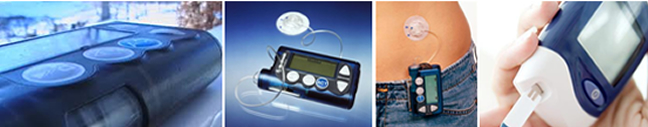
\includegraphics[scale=1]{images/bombainsulina.png}
	\caption{Imagens de uma bomba de infusão de insulina}	
	\label{fig:bombainfusao}	
\end{figure}


Seu funcionamento é bem simples, libera-se uma quantidade de insulina, programada pelo médico, durante o dia todo, simulando o funcionamento do pâncreas de uma pessoa saudável, entretanto existem cuidados a serem tomados: calcular a quantidade de carboidratos ingeridos a cada refeição e programar o aparelho para injetar uma quantidade de insulina com maior velocidade no organismo nos horário em que se faz as refeições principais.
Quanto a quem pode usar, a pessoa deve cumprir alguns pré-requisitos que são:
\begin{itemize}
\item Conseguir medir o índice glicêmico no mínimo 4 vezes por dia;
\item Durante a fase de adaptação e ajuste da dosagem a serem utilizadas pela bomba, fazer a medição glicêmica de 6 a 8 vezes por dia;
\item Seguir as recomendações médicas além de manter contato e um constante \emph{feedback} com os responsáveis pela bomba e, além de tudo, seguir a dieta recomendada, respeitando quantidades ingeridas;
\item Ter condição financeira para custear o equipamento e o contato com os responsáveis por ele;
\item Estar disposto ao uso da bomba durante o dia todo, 24 horas junto ao corpo;
\item Aprender sobre contagem de carboidratos para saber seu consumo durante as refeições;
\item Praticar exercícios.
\end{itemize}

Cumprindo os pré-requisitos citados temos as vantagens de seu uso que são:

\begin{itemize}
\item Maior flexibilidade no horário das refeições;
\item Se usada corretamente o risco de hipoglicemia é reduzido, e a longo prazo as complicações devido ao diabetes também;
\item Melhora o controle glicêmico;
\item Melhora no controle do fenômeno do amanhecer, responsável pelo aumento do índice glicêmico durante a manha, entre as 4 e 8 horas da manha, causador da hipoglicemia se o diabético não calculou a dose de insulina antes de dormir, ou não se levantou durante a noite para gerenciá-la.
\end{itemize}

Mas mesmo com todas as vantagens dada devido ao uso do equipamento caso o diabético seja obeso, ingira grandes quantidades de alimento ou açúcar, ou seja, carboidratos, não praticar atividades físicas, não fazer a medição do índice glicêmico na quantidade de vezes recomendada, ou até mesmo determinar por si só a quantidade de insulina a ser utilizada, não existe vantagem no seu uso.
É importante ter em mente que mesmo com toda facilidade e tecnologia existente o acompanhamento médico não deve ser deixado de lado. As principais indicações médicas para o uso do equipamento são:

\begin{itemize}
\item Fenômeno do amanhecer;
\item Hipoglicemia;
\item Diminuir a variação do índice glicêmico;
\item Hiperglicemia;
\item Recorrente ceatosidade, que é o acumulo de ceatócidos, pois o fígado quebra a gordura e proteína devido à falta de insulina, pois o corpo não consegue utilizar a glicose como energia;
\item Flexibilidade, especialmente para crianças pequenas;
\item Gestação, viagens e atividade físicas;
\item Fobia de injeção;
\item Desejo do diabético \cite{diabetes2013, portaldiabetes2009}.
\end{itemize}

\section{Motivação}
Segundo a Sociedade Brasileira de Diabetes \cite{sbc2014}, diversos estudos realizados mostram que o tratamento feito através da Infusão de insulina tem diversas melhorias quando comparado com outros tratamentos existentes. Entretanto não é o mais utilizado devido ao seu alto custo, devido a importação.
Logo, esse projeto vem com foco social: facilitar o acesso da população brasileira de baixa renda ao equipamento, melhorando sua qualidade de vida dos portadores da doença que se encaixem nesse perfil. 

\section{OBJETIVOS}
Esse projeto tem como objetivo principal desenvolver um software para um protótipo de uma Bomba de Infusão de insulina utilizando o microcontrolador da família PIC, PIC18F452. 

\subsection{OBJETIVOS SECUNDÁRIOS}

Em segundo plano este trabalho foca em:
\begin{itemize}
\item Aprendizado sobre as características e funcionalidades disponíveis do microcontrolador escolhido;
\item Aprendizado das tecnologias utilizadas como: compilador, simulador e bibliotecas disponíveis;
\item Desenvolvimento das funcionalidades básicas de uma bomba de infusão de insulina;
\item Aprendizado sobre a escolha e uso de um motor de passo;
\item Aprendizado sobre a forma de uso de um \emph{display} de LCD para comunicação com o usuário.
\end{itemize}

\section{PROCEDIMENTOS METODOLÓGICOS}
Este trabalho foi dividido em duas etapas: pesquisa para levantamento de referências bibliográficas e desenvolvimento prático. Durante a primeira etapa, foi feita a pesquisa e levantamento bibliográfico sobre o tema em questão para que fosse possível um melhor entendimento da plataforma, tecnologias e, claro, do problema abordado. Juntamente com essa pesquisa, foi feito um estudo sobre o microcontrolador PIC escolhido, PIC18F452, a partir do material encontrado. O estudo e desenvolvimento foi feito utilizando o compilador MikroC e sua IDE, já para os testes utilizou-se o simulador Proteus. Em seguida houve-se um levantamento de informações sobre sistemas embarcados, sistemas críticos e sistemas críticos de tempo real, e assim adquirindo-se conhecimento sobre os conceitos de desenvolvimento da área em questão, uma vez que a confiabilidade e segurança do problema proposto é importantíssimo.


O software de controle do protótipo da bomba de infusão de insulina foi desenvolvido na linguagem C, compilado para o microcontrolador já citado, PIC18F452. O sistema é responsável basicamente por gerenciar o perfil de infusão basal, calcular intervalos corretos e passos necessários para uma infusão. Desta forma, o
software foi dividido nos seguintes módulos: Config, LCD, InsulinPump, Motor, Menu, TimerMotor e principal. 

Essa divisão por módulos é, e foi, extremamente importante para o desenvolvimento do sistema. Somando-a à um dos conceitos mais importante desse projeto - OOC, \emph{Object-Oriented Programming With ANSI-C} - são as chaves para a facilidade de manutenção, entendimento do código e possível evolução do projeto.

As responsabilidade dos módulos são bem claras e isoladas:

Config: Centralizar configurações gerais do sistema;
LCD: Abstrair uso do periférico para o resto do sistema;
InsulimPump: Abstrair funcionamento, requisitos de segurança e outras particularidades da bomba;
Motor: Abstrai como se controla o motor e qual tipo está sendo utilizado para infusão;
TimerMotor: Separa o gerenciador de tempo das particularidade únicas do hardware e compilador;
Menu: Facilitar navegação entre menus, simulando máquina de estado;
Principal: Possui o \emph{loop} principal para navegação simples entre os menus existentes.

E, finalizando, após o desenvolvimento, executou-se uma bateria de testes para se o funcionamento da bomba estava sendo de acordo coma forma especificada, levando em conta toda a integração necessária com os periféricos existentes.


% ----------------------------------------------------------
% Sistemas Embarcados
% ----------------------------------------------------------
\chapter{SISTEMAS EMBARCADOS}
Sistema embarcado em geral é uma combinação de \emph{hardware} e \emph{software} para executar uma tarefa específica diferente dos computadores do dia-a-dia que possuem inúmeros propósitos: verifica e-mail, escrever monografias, entre outros. Sistemas embarcados podem possuir ou não um sistema operacional, seja um RTOS, possui requisitos de tempo de execução, ou um Linux e, portanto, pode ser desenvolvido em um \emph{hardware} com microcontrolador ou microprocessador \cite{wikibook2012embedded}.

Segundo \cite{cunha2013} a inteligência embarcada é uma tendência futura, cada vez mais inteligência será adicionada aos equipamentos do dia-a-dia, considera que um micro-ondas atual tem mais capacidade computacional do que tinha o projeto Apolo, que levou o homem a lua. Esta crescente utilização se dá basicamente pelo preço e consumo reduzido dos microcontroladores, além da grande flexibilidade ao atender os mais diversos problemas visto o vasto número de arquiteturas disponíveis: ARM, MIPS, Coldfire/68k, PowerPC, x86, PIC, 8051, Atmel AVR, Renesas H8, SH, V850, FR-V, M32R, Z80, Z8 e outras. Um contraste que atrai diversos desenvolvedores quando comparado com o número limitado de arquiteturas diponíveis para microprocessadores do mercado de computadores pessoais \cite{germano2011}.

A comunicação dos microcontroladores com o meio externo, segundo \cite{germano2011}, se dá pelos periféricos e o mais comuns são:
\begin{itemize}
\item Entrada de dados através de teclas, geralmente pelo de teclados feitos com varredura matricial;
\item \emph{Leds};
\item \emph{Display’s} de LCD, sendo os mais comuns os alfanuméricos como o HD44780;
\item Interface serial, por exemplo RS232 e I2C;
\item USB, \emph{Universal Serial Bus};
\item TCP/IP.
\end{itemize}

Como dito anteriormente, esses sistemas estão cada vez mais no dia-a-dia das pessoas e, claro, facilitando a vida delas, mas muitas vezes não são percebidos. E cada vez mais estão mais acessíveis podendo automatizar funções até mesmo dentro das próprias casas. A Figura \ref{fig:exemplosistemasembarcados}\footnote{\url{http://bytesdontbite.com/2012/06/26/embedded-systems-no-bdb/}} mostra alguns sistemas embarcados e onde são utilizados:

\begin{figure}[htp]
	\centering
	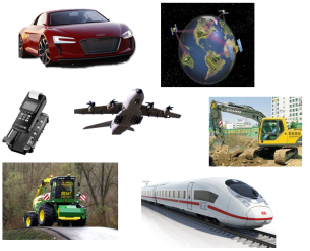
\includegraphics[scale=1]{images/exemplo_sistemas_embarcados.png}
	\caption{Exemplo de Sistemas embarcados}	
	\label{fig:exemplosistemasembarcados}	
\end{figure}

\section{SISTEMAS EMBARCADOS DE TEMPO}
O conceito Tempo Real é complexo para ser explicado, mas sua ideia básica é que se espera que o computador responda algo para o ambiente externo em tempo. Normalmente pessoas assumem que tempo real significa "muito rápido", entretanto não é verdade, tempo real simplesmente significa "rápido o suficiente" no contexto de operação do sistema. Um exemplo é a ação do motor, pode-se dizer que é "rápida", pois o sistema deve tomar decisões como - fluxo de combustível, tempo da faísca - toda vez que o motor completa um ciclo.

Sistemas de tempo real são baseados em previsibilidade e, segundo \cite{farines2000sistemas}, essa previsibilidade de um sistema de tempo real é obtida quando independente de falhas, sobrecargas e variações de hardware, e assim é possível que seu comportamento seja antecipado antes de sua execução. Isso tem a finalidade de poder prever o funcionamento de um sistema de tempo real e garantir as suas restrições temporais, e para isso é necessário definir hipóteses em relação a carga e falhas em relação ao ambiente externo deste sistema \cite{farines2000sistemas}. 
Segundo \cite{mall2009real} os sistemas de tempo real são classificados em dois tipos:
\begin{itemize}
\item \emph{Soft Real Time Systems}: Sistemas não críticos de tempo real, onde a ocorrência de uma falha temporal é da mesma ordem de grandeza que os resultados em que o funcionamento está correto, exemplos: Máquina de lavar e portão eletrônico de uma casa;
\item \emph{Hard Real Time Systems}: Sistemas Críticos de Tempo Real, onde a ocorrência de uma falha temporal complicam, e muito, os resultados quando comparado com seu funcionamento correto, exemplos: sistema de controle de um avião e um sistema de controle de semáforos.
\end{itemize}

\section{SISTEMAS EMBARCADOS CRÍTICO}
\label{sec:SistemaEmbarcado}

Sistema Crítico é um sistema no qual a confiança é fundamental, ou melhor, a questão mais importante em seu desenvolvimento. Isso porque sistemas críticos, em caso de falha, podem causar consequências gravíssimas para os humanos, economia e outras áreas. Pode-se dizer que seus indicadores são: Disponibilidade, confiabilidade, segurança e proteção. E para que essa confiança seja alcançada deve-se evitar erros durante seu desenvolvimento e realizar diversos testes para que seja possível detectar e corrigir os erros que passarem de forma que seja possível limitar os danos causados por falhar operacionais \cite{sommerville2004software,feldmann2007survey,jordan2006standard}.

Segundo \cite{kopetz2011real} as classificações dos sistemas embarcados críticos podem ser:
\begin{itemize}
\item \emph{Fail Safe}: Classificação para sistemas onde o estado seguro pode ser atingido em caso de falha, como por exemplo, esgotar a bateria de uma bomba de insulina;
\item \emph{Fail Operational}: Classificação para sistemas que em caso de falhas ainda são capazes de fornecer algum tipo de serviço, mesmo que mínimo. Um exemplo é um sistema de controle de voo que, mesmo em caso de falha, é capaz de fornecer serviços e ser seguro.
\end{itemize}

Abaixo a Figura \ref{fig:exSistEmbarcado},  mostra exemplos de sistemas embarcados críticos.

\begin{figure}[htp]
	\centering
	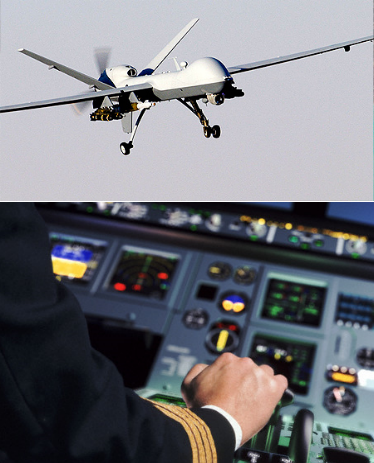
\includegraphics[scale=0.7]{images/exemplo_sistemas_embarcados_criticos.png}	
	\caption{Sistemas embarcados críticos}
	\label{fig:exSistEmbarcado}	
\end{figure}

\section{MICROCONTROLADOR}
Microcontroladores são chips inteligentes que utilizam a arquitetura Harvard, RISC. É constituído basicamente por pinos de entradas e saídas e memória. Suas saídas podem ser controladas através de programação e em função do processamento de suas entradas. Sua programação pode ser feita em diversas linguagens como: C, C++, entre outras \cite{radio2012amadores}.

Segundo \cite{ganssle1999art}, o microcontrolador é a parte mais importante de um sistema embarcado e sua principal diferença quando comparada com um microprocessador é o fato de ser um sistema computacional completo que integra todos as principais partes da arquitetura de Von Neumann em um único componente, as partes citadas são:
\begin{itemize}
\item CPU: \emph{Central Processor Unit};
\item Memória RAM: \emph{Random Access Memory};
\item Portas I/O: Portas de entrada e saída.
\end{itemize}

Além de ser composto por temporizadores, memória ROM (\emph{Read Only Memory}), conversor AD, analógico – digital, e DA, digital – analógico.
Comparados com microprocessadores, os microcotroladores possuem consumo e \emph{clock}, processamento, reduzidos, isso devido ao fato que o primeiro é destinado a tarefas que necessita uma alta capacidade de processamento como, por exemplo, os microprocessadores do nosso PC do dia-a-dia. Por padrão, os microprocessadores são utilizados em situações que os requisitos são abrangentes, com entradas e saída variadas como: sensores, atuadores e periféricos de comunicação \cite{lee2011introduction}.

\subsection{PIC}
PIC é um circuito integrado produzido pela \emph{Microchip Technology Inc}. Seu nome significa: \emph{Programmable Interface Controller}, Controlador de Interface Programável. Externamente possui uma aparência de um circuito integrado mais comuns - TTL ou CMOS -, mas na verdade contém todos os componentes de um sistema microprocessado como: CPU, \emph{Central Processor Unit}, sua finalidade é interpretar as instruções de programa; Memória PROM, \emph{Programmable Read Only Memory}, na qual memorizará as instruções do programa; Memória RAM, \emph{Random Access Memory}, utilizada pra memorizar as variáveis do programa; Linhas de I/O, entrada e saída, para controlar dispositivos internos e receber informações do meio externo; entre outros \cite{radio2012amadores,wikipedia2012pic}.

\subsection{SENSORES}
A definição de sensor pode ser a de um transdutor capaz de alterar sua característica física interna em resposta à um fenômeno físico externo. Além disso, existem sensores considerados de operação indireta que são os quais alteram suas propriedades como capacitância, resistência, ou, até mesmo, sua indutância, sob ação de algum gradeza ou evento externo \cite{rosario2006principios}. 

Segundo \cite{nomadusp2014}, os sensores são largamente utilizados na medicina, indústria, robótica, além de outras aplicações. Considerando que o sinal é sempre uma forma de energia, os sensores podem ser classificados em função da energia que é capaz de detectar, como:

\begin{itemize}
\item Sensores de luz: células solares, fotodíodos, fototransistores, tubos fotoelétricos, e outros;
\item Sensores de som: microfones e hidrofone;
\item Sensores de temperatura: termômetros e termopares;
\item Sensores de resistência elétricas: ohmímetro. 
\item Outros;
\end{itemize}

\subsection{SENSORES BIOLÓGICOS}
Segundo \cite{nomadusp2014}, os sensores citados anteriormente são corretamente chamados de sensores artificiais. Isto devido ao fato de existir sensores naturais ou biológicos, já que todos os organismos vivos possuem sensores capazes de agir da mesma forma que os artificias. Esses sensores biológicos são células especializadas, sensíveis a:

\begin{itemize}
\item Luz, movimento, temperatura, vibração, pressão, campos eléctricos, som, e outros aspectos físicos do ambiente;
\item Grande variedade de moléculas ambientais, incluindo toxinas e nutrientes;
\item Aspectos metabólicos, tais como os níveis de glicose e oxigênio;
\item Até mesmo as diferenças entre proteínas do ambiente externo e do próprio organismo.
\end{itemize}

Esses sensores artificiais que imitam sensores biológicos, utilizando componentes biológicos, são chamados biossensores.

\subsection{ATUADORES}
Segundo \cite{chironis1991mechanisms}, dispositivos considerados atuadores são aqueles que transformam uma forma de energia em outra, causando mudanças no ambiente em que estão atuando, ou seja, de acordo com sinais, ou impulsos, recebidos realizam ações capazes de alterar as grandezas físicas do ambiente em questão. Eles são capazes de converter energias como: energia elétrica, hidráulica e pneumática em energia mecânica. Segue exemplos de alguns tipos de atuadores:

\begin{itemize}
\item Atuadores eletromagnéticos: São os motores elétricos como motores de passos, servos;
\item Atuadores hidráulicos: Utilizam um fluido submetido a uma pressão para movimentar um braço, são utilizados em robô que operam grandes cargas;
\item Atuadores pneumáticos: Utilizam um gás submetido a uma pressão para movimentar o braço, possuem menor custo que os hidráulicos, sendo utilizados em robôs de menor porte;
\end{itemize}

\subsection{MOTOR DE PASSO}
Motor de passo é um dispositivo eletromecânico. Sua principal propriedade é sua habilidade de transformar pulsos elétricos em movimentos, que são precisamente incrementados na posição do rotor e são denominados "passos". Esse tipo de motor é caracterizado como máquina duplamente saliente, significando que possui dentes, compostos por matérias magnéticos nas duas partes que o compõe: A parte imóvel chamada estator e a móvel rotor \cite{demotor, acarnley2002stepping}.

Seu uso é interessante em situações em que precisão nos movimentos é necessária. Isso porque com ele é possível controlar: ângulo de rotação, velocidade, posição e sincronismo. Suas vantagens não são seu torque nem a capacidade de gerar movimentos de alta velocidade, mas sim a precisão em seus movimentos. Devido a essas características esse tipo de motor é amplamente utilizado em: câmeras de vídeo, robôs, brinquedos, \emph{scanners}, impressoras, entre outros \cite{demotor}.

De forma simples o funcionamento de um motor de passo consiste no uso de materiais magnéticos, ou solenoides, como dito anteriormente, alinhados dois a dois, representando os polos norte e sul, que quando energizados atraem o rotor fazendo-o se alinhar as partes energizadas do estator, causando assim um pequeno movimento: o passo. Sua velocidade e sentido estão diretamente relacionados à forma com que os solenoides são acionados, o primeiro com a frequência e o segundo a ordem de acionamento \cite{demotor, acarnley2002stepping,wikipedia2012stepper}.

\subsection{MOTOR DE PASSO RELUTÂNCIA VARIÁVEL – \emph{MULTI STACK}}
A fonte do fluxo magnético desse tipo de motor são as bobinas colocadas nos dentes do estator. O acionamento das bobinas é feito em sequência para incentivar o movimento, alinhamento, dos conjuntos de dentes sucessivos do estator e do rotor dando ao motor a característica de passos. Ao longo de eu eixo ele é dividido em seções isoladas magneticamente chamadas \emph{stacks}, daí o nome \emph{multi stack}, e cada uma pode ser excitada por uma bobina separadamente chamada phase. Cada \emph{stack} possui um estator, preso em sua posição pela caixa, suporte, do motor junto com as bobinas e o elemento móvel, rotor.

O rotor é uma unidade única e maciça que será utilizado para a movimentação da carga. O material do rotor é um metal elétrico laminado o que permite que o campo magnético possa mudar rapidamente sem grandes perdas. O estator de cada rotor possui um determinado número de polos e uma parte da \emph{phase}, bobina, é enrolada em torno de cada polo para produzir o campo magnético. Os polos adjacentes são enrolados no sentido oposto assim os campos magnéticos adjacentes possuem sentidos opostos. Com isso o circuito magnético completo é considerado um polo do estator, o dente do rotor, o vão de ar entre os dentes de ambos e, por fim, um polo adjacente do estator. E esse circuito é repetido a cada par de polos do estator. As forças normais produzidas pelos polos do estator e os dentes do rotor são iguais e se anulam assim sobra apenas a força tangencial o que causa o movimento, isso pode ser visto conforme a Figura ~\ref{fig:forcamotorpassobainfusao}.

\begin{figure}[htp]
	\centering
	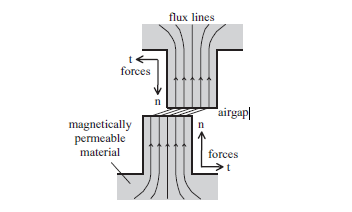
\includegraphics[scale=1]{images/forca_motor_passo.png}
	\caption{Forças normais e tangenciais}	
	\label{fig:forcamotorpassobainfusao}	
\end{figure}

A posição do rotor com relação ao estator é ajustada toda vez que as bobinas são excitadas. O ajuste ocorre, pois os dentes de ambos são alinhados o que tende a diminuir a relutância do circuito magnético, daí surgiu o nome do motor. Considerando a Figura ~\ref{fig:visaomotorpasso} é possível perceber que para girar no sentido horário a ordem de acionamento deve ser A, B, C, A, B, C, A... e no sentido anti-horário A, C, B, A, C, B, A...

\begin{figure}[htp]
	\centering
	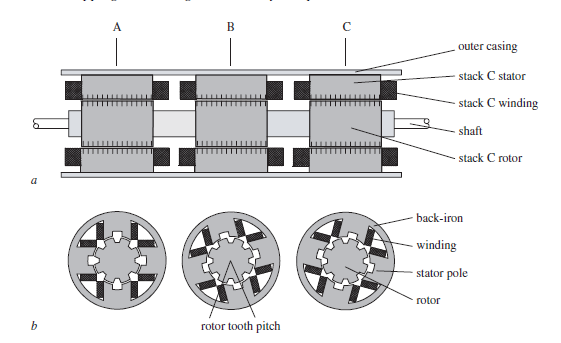
\includegraphics[scale=1]{images/visao_motor_passo.png}
	\caption{Visão paralela e perpendicular das \emph{stacks} e rotor}	
	\label{fig:visaomotorpasso}	
\end{figure}

\newpage Segundo \cite{acarnley2002stepping}, existe uma pequena relação entre o comprimento do passo. Considere N o número de dentes do estator e p o número de dentes do rotor logo: 

\begin{equation}
  \emph{step length} = 360/(N * p)
\end{equation}

\subsubsection{\emph{DESIGN} DO MOTOR}
Cada polo do estator produz um campo magnético quando excitado com uma corrente DC. A performance do motor depende da força do campo magnético gerado pelas bobinas quando excitadas, logo o campo magnético está diretamente ligado ao torque do motor. A força do campo magnético está relacionada à intensidade da corrente que passa pelas bobinas, portanto em teoria aumentar a corrente para aumentar o torque seria o suficiente, entretanto existe um limitante que é o aumento da temperatura nas bobinas.

No exemplo da Figura ~\ref{fig:visaomotorpasso} cada \emph{stack} tem 4 polos. Uma vez que todas as quatro bobinas devem ser excitadas concorrentemente uma prática comum é interconectar as bobinas para formar apenas uma \emph{phase}. A forma com que as bobinas são interconectadas influência na temperatura que será dissipada pela bobina uma vez que isso está diretamente ligada à intensidade da corrente. A potência não varia conforme a interconexão. 

Existem 3 formas de interconexão conforme a Figura ~\ref{fig:bobinas}. Na verdade a potência não varia conforme a interconexão, mas sim qual \emph{driver} de controle será utilizado: baixa voltagem e alta corrente com uma conexão paralela ou alta voltagem e baixa corrente com uma conexão em série. A diferença entre as 3 interconexões pode ser vista na Figura ~\ref{fig:relacaobobina} \cite{acarnley2002stepping}.

\begin{figure}[htp]
	\centering
	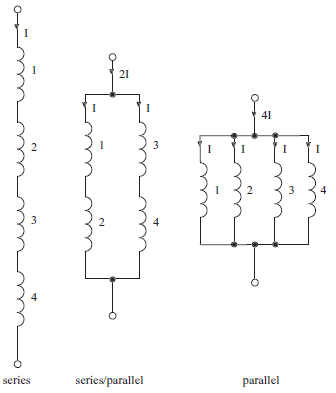
\includegraphics[scale=1]{images/bobinas.png}
	\caption{Interconexão das bobinas}	
	\label{fig:bobinas}	
\end{figure}

\begin{figure}[htp]
	\centering
	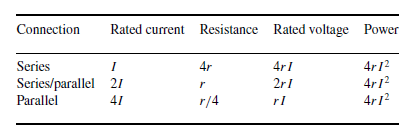
\includegraphics[scale=1]{images/relacao_bobina.png}
	\caption{Relação das interconexões das bobinas}	
	\label{fig:relacaobobina}	
\end{figure}

\subsection{MOTOR DE PASSO RELUTÂNCIA VARIÁVEL – \emph{SINGLE STACK}}
Como o nome já diz esse motor é construído com apenas uma stack, ou melhor, uma unidade. Entretanto quanto ao funcionamento e princípios básicos é idêntico ao \emph{multi stack}. Cada dente do estator ainda possui uma bobina separada que produz um campo magnético quando excitada por uma corrente DC.

Uma mudança é que as bobinas do lado oposto são conectadas para formar uma phase. Na Figura ~\ref{fig:singlestack} existe 3 phases que é o número mínimo para poder rotacionar para os dois lados. A bobina no dente oposto no estator está no sentido oposto para que sejam gerados campos magnéticos em sentidos opostos. E por fim a relação de comprimento do passo se mantém conforma o motor \emph{multi stack} \cite{acarnley2002stepping}.

\begin{figure}[htp]
	\centering
	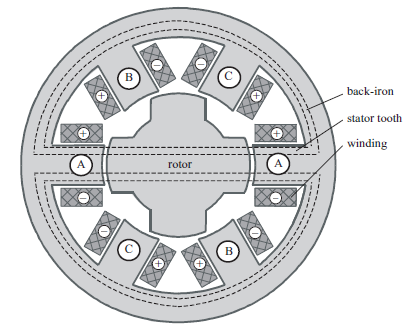
\includegraphics[scale=1]{images/single_stack.png}
	\caption{\emph{Stator single stack}}	
	\label{fig:singlestack}	
\end{figure}

\subsection{MOTOR DE PASSO HÍBRIDO}
A diferença principal desse com os tipos anteriores é que o circuito magnético é excitado por uma combinação de bobinas e imã permanente. Seu funcionamento e princípios básicos são idênticos ao \emph{multi} e \emph{single stack}. As bobinas ainda permanecem nos dentes do estator já o imã compõe o eixo do rotor conforme Figura ~\ref{fig:hibrido}.

\begin{figure}[htp]
	\centering
	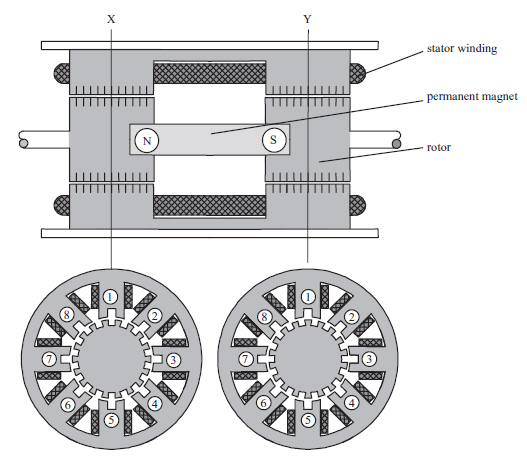
\includegraphics[scale=0.7]{images/hibrido.png}
	\caption{Motor híbrido}	
	\label{fig:hibrido}	
\end{figure}

Existem duas bobinas, \emph{phases}, situadas em 4 dos 8 polos do estator, conforme Figura \ref{fig:hibrido}. A bobina A está nos polos 1, 3, 5, 7 e a B nos polos 2, 4, 6, 8. Polos adjacentes ainda são envolvidos pelas bobinas em sentidos opostos, portanto se a bobina A é alimentada com corrente positiva o campo magnético é direcionado para fora nas bobinas 3 e 7, mas para dentro nos polos 1 e 5 e o mesmo acontece na bobina B.

Quando se aplica corrente nas bobinas a mesma ideia de alinhamento dos dentes do rotor e stator acontece. Considerando a Figura \ref{fig:hibrido} e o exemplo da excitação positiva na bobina A, citada anteriormente, o estator e o rotor são alinhados sob os polos 3 e 7 na seção X e polos 1 e 4 na seção Y.

Para uma rotação continua o motor necessita de uma excitação sequencial das bobinas. Se retirar a excitação de A e colocar em B o alinhamento dos dentes vai acontecer com 4 e 8 na seção X e 2 e 6 na seção Y. Isso faz com que o motor gire no sentido horário, a sequência deve ser A+, B+, A-, B-,... Para o sentido anti-horário A+, B-, A-, B+.

Segundo \cite{acarnley2002stepping}, a relação de comprimento do passo é similar ao de relutância variável. Existe uma relação com o número de dentes do rotor p, e com um ciclo completo de excitação. Como um esse ciclo em um motor hibrido consiste em 4 estados e produz 4 passos de movimento no rotor, logo conclui-se que:
\begin{equation}
  \emph{step length} = 360/(4 * p) = 90 / p
\end{equation}

\subsection{COMPARAÇÃO ENTRE TIPOS DE MOTORES}
Não é possível dizer categoricamente que um motor é melhor do que o outro em todas as situações. Os híbridos têm menor comprimento de passo, normalmente 1,8 graus, o que pode ser uma grande vantagem quando alta precisão é necessária. Eles também possuem maior torque devido ao uso do imã permanente no rotor. E, além disso, quando nenhuma bobina esta excitada o motor hibrido ainda possui um "torque de retenção" que mantém a posição do rotor. E isso pode ser uma característica na aplicação onde a posição do rotor deve ser preservada durante uma falha de energia, mas é bom lembra que esse torque é menor do que o torque com 1 ou mais bobinas excitadas.

Já o de relutância variável tem duas vantagens quando se trata de movimentar carga em distâncias consideráveis. A primeira é que tipicamente o comprimento de seu passo é de 15 graus, maior que o do híbrido, portanto ele precisa de menos passos para mover a mesma distância. Com a redução do número de excitações das bobinas o consumo também é reduzido, em caso de uso de baterias é uma característica muito interessante. A segunda é que por não possuir imã permanente possui uma menor inércia para início de movimento, também diminuindo o consumo inicial \cite{acarnley2002stepping}.

\subsection{LCD - \emph{Liquid Crystal Display}}
Um \emph{display} de cristal líquido, LCD, é utilizado para exibir informações como texto, imagens e vídeos. É composto por um painel fino e, segundo \cite{lcd1996unicamp}, é um componente, considerado interface de saída, muito utilizados em conjunto com microcontroladores. Exemplos de uso são: \emph{cockpit} de aeronaves, \emph{displays} em computadores de bordo de automóveis, dispositivos de jogos, relógios, calculadoras e outros.

Pode-se classificar os módulos de LCD em: exibição gráfica e exibição de caractere. Os módulos gráficos são encontrados com resoluções de 122x32, 128x64, 240x64 e 240x128 pixel, possuindo, geralmente, 20 pinos para conexão. Já os modelos comuns, tipo caractere, tem sua especificação em função dos números de linhas e colunas, a Figura \ref{fig:pinoslcd} representa seus sexemplos.

\begin{figure}[htp]
	\centering
	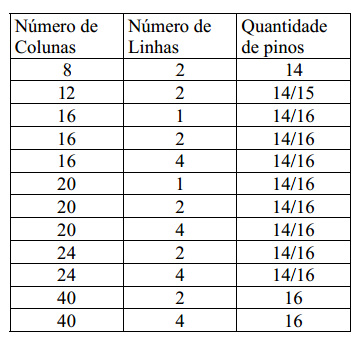
\includegraphics[scale=1]{images/tabelas_pinos_lcd.png}
	\caption{Tabelas de pinos LCD comum}	
	\label{fig:pinoslcd}	
\end{figure}

% ----------------------------------------------------------
% Proteus
% ----------------------------------------------------------
\chapter{PROTEUS \emph{DESIGN SUITE}}
Proteus é um suíte, conjunto de \emph{features}, desenvolvido pela Labcenter Eletronics Ltd. É um software para: simulação de microcontroladores, simulação de circuitos eletrônicos e para desenvolvimento de placa de circuito impresso. Os componentes desse sistema são:
\begin{itemize}
\item ISIS \emph{Schematic Capture}: Ferramenta utilizada para se adicionar objetos, componentes para simulação;
\item PROSPICE \emph{Mixed mode SPICE simulation}: Simulador industrial padrão SPICE3F5, combinado com simulador digital de alta velocidade. \emph{Spice, Simulation Program with Integrated Circuit Emphasis}, é um simulador para propósitos gerais para sistemas eletrônicos analógicos.
\item ARES PCB \emph{Layout}: Sistema de PCB, \emph{Printed Circuit Board}, ou melhor, placa de circuito impresso, design de alto desempenho com posicionamento automático de componente, auto-roteamento, entre outras \emph{features} relacionadas ao desenvolvimento de placas de circuito impresso.
\item VSM - \emph{Virtual System Modelling}: Permite simular software embarcado para microcontroladores, disponíveis em suas bibliotecas, ao lado de seu projeto de hardware \cite{proteus2013, wikipedia2012spice}.
\end{itemize}

\section{ISIS \emph{SCHEMATIC CAPTURE}}
Como já foi dito, essa feature se trata da funcionalidade de simulação e montagem de circuitos eletrônicos. Permite que o circuito em questão seja debugado de forma simples e, além disso, possibilita uma integração com códigos desenvolvidos para microcontroladores suportados por ele. Seus componentes são:

\begin{itemize}
\item Circuitos integrados das famílias: 74ALS, 74AS, 74F, 74HC, 74HCT, 74LS, 74S e 74STD;
\item Componentes analógicos;
\item Medidores de corrente e tensão para serem utilizados durante o debug;
\item Geradores como fontes e clock, ambos ajustáveis para o valor desejado;
\item Semicondutores como diodo, transistor, LEDs e outros;
\item Componentes básicos como chaves, resistores, capacitores e indutores;
\item Atuadores como motor DC, motor de passo e outros;
\item Microcontroladores da família 80XXX, AT e PIC;
\item Memórias, displays, CMOS e outros.
\end{itemize}

Seu uso é bem simples, pois é como se estivesse desenhando o circuito em um papel. Após ser desenhado é possível utilizar as ferramentas de auxilio para debug e assim coletar dados como voltagem e corrente do circuito e até mesmo se o funcionamento está conforme o esperado.

% ----------------------------------------------------------
% MikroC
% ----------------------------------------------------------
\section{MIKROC}
MikroC é um \emph{toolchain} poderoso, uma ferramenta de desenvolvimento completa para microcontroladores da família PIC. Criado de forma que disponibilize ao usuário a forma mais fácil de desenvolver suas aplicações para sistemas embarcados, sem compromisso de desempenho ou controle. MikroC permite que seja feito um rápido desenvolvimento e embarcar aplicações complexas:

\begin{itemize}
\item Escrever códigos em C utilizando um editor de código avançado;
\item Utilizar as bibliotecas do próprio MikroC para acelerar o desenvolvimento: aquisição de dados, memória, \emph{display}, comunicação, entre outros;
\item Auxilia na evolução e desenvolvimento do código monitorando a estrutura do programa, variáveis e funções. Gera um código comentado, humanamente legível em assembler, e um padrão HEX compatível com o padrão conhecido;
\item Possui um \emph{debugger} integrado capaz de gerar relatórios detalhados, estatísticas, pilha de execução, entre outras opções que auxiliam analisar o fluxo do programa \cite{mikroc2006}.
\end{itemize}

% ----------------------------------------------------------
% PIC18F452
% ----------------------------------------------------------
\section{PIC18F452}
O PIC18F452 é um microcontrolador fabricado pela empresa \emph{Microchip Technology}. Possui tecnologia CMOS, como consequência tem um consumo baixíssimo, possui memória do tipo FLASH, um grande facilidade para desenvolvimento de protótipos, uma vez que para apagá-la não é preciso utilizar luz ultravioleta como em versões antigas, utilizavam memória EEPROM. Abaixo seguem as principais características desse microcontrolador:

\begin{itemize}
\item Microcontrolador de 40 Pinos;
\item Memória de programa FLASH de 32Kbytes;
\item Memória RAM de 1536 bytes;
\item Memória EEPROM de 256 bytes;
\item Processamento de até 10MIPS;
\item Quatro \emph{timers}, ou temporizadores, internos – um de 8 bits e 3 de 16 bits – TIMER0, TIMER1, TIMER2 e TIMER3;
\item 2 canais capture/compare/PWM – Módulo CCP;
\item Módulo \emph{Master Synchronous Serial Port} (MSSP);
\item \emph{Unhaced Usart;}
\item 8 canais A/D de 10 bits;
\item Detector de baixa voltagem programável;
\item Permite até 100.000 ciclos de escrita e leitura na memória FLASH;
\item Permite 1.000.000 ciclos de escrita e leitura na memória EEPROM.
\item Retenção de dados na FLASH por 40 anos;
\item \emph{Watchdog timer} com oscilador próprio e programável;
\item Três pinos de interrupções externas: INT0, INT1 e INT2
\end{itemize}

A Figura \ref{fig:pic} representa uma imagem do microcontrolador.

\begin{figure}[htp]
	\centering
	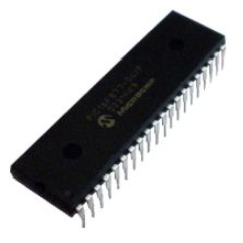
\includegraphics[scale=1]{images/pic.png}
	\caption{PIC18F452}	
	\label{fig:pic}	
\end{figure}

\newpage 
\subsection{Estrutura Interna}
A Figura \ref{fig:estuturapic} ilustra como é a estrutura interna do microcontrolador:

\begin{figure}[htp]
	\centering
	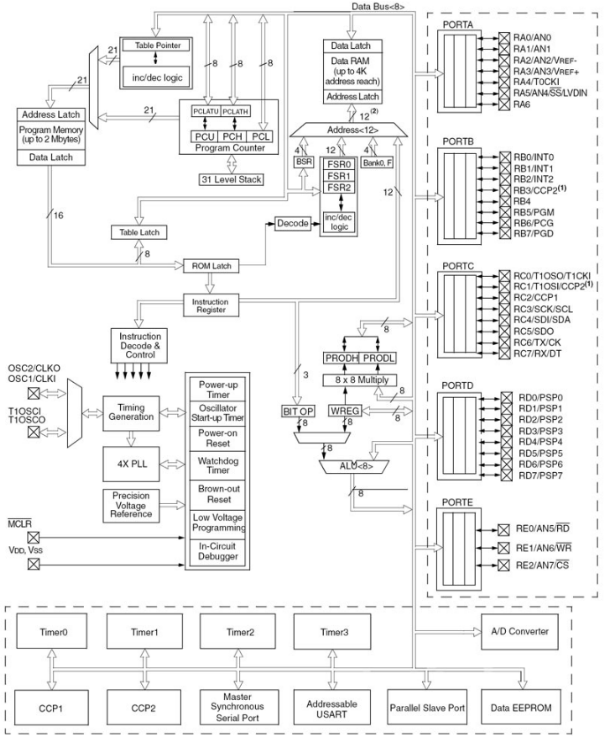
\includegraphics[scale=0.6]{images/estrutura_pic.png}
	\caption{Estrutura Interna PIC18F452}	
	\label{fig:estuturapic}	
\end{figure}

\newpage 
\subsection{DESCRIÇÃO DOS PINOS}
Dos 40 pinos desse microcontrolador 34 são pinos I/O, entrada e saída, divididos em 5 "PORT". A Figura \ref{fig:pinospic} representa uma relação dos pinos do microcontrolador.

\begin{figure}[htp]
	\centering
	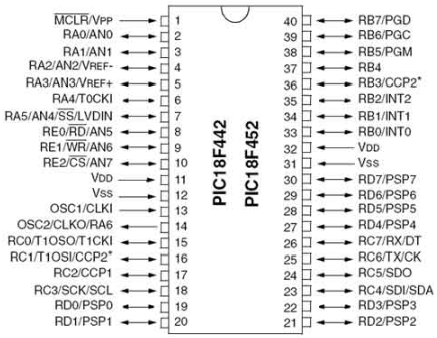
\includegraphics[scale=0.6]{images/pinos_pic.png}
	\caption{Pinos PIC18F452}	
	\label{fig:pinospic}	
\end{figure}

A divisão dos pinos I/O citada é da seguinte maneira:

\begin{itemize}
\item PORTA: São 7 pinos nomeados de RA0 a RA6. Podem ser utilizados como I/O geral ou conversor A/D, essa segundo opção tem exceção o pino RA4. Além de possuir a opção LVD, detecção de baixa tensão;
\item PORTB: São 8 pinos nomeados de RB0 a RB7. Podem ser utilizados para I/O geral e, além disso, pode-se trabalhar com três interrupções externas, módulo CCP, pinos de gravação e debug;
\item PORTC: São 8 pinos nomeados de RC0 a RC7. Podem ser utilizados para I/O geral, saída do oscilador do \emph{timer}, módulo CCP, Clock e data(dados) para os modos SPI, I2C e UART;
\item PORTD: São 8 pinos nomeados de RD0 a RD7. Podem ser utilizados para I/O geral ou como PSP para ter saída TTL, para interfaceamento com microprocessadores, por exemplo;
\item PORTE: São 3 pinos nomeados de RE0 a RE2. Podem ser utilizados para I/O geral ou pinos de controle de acesso.
\end{itemize}

% ----------------------------------------------------------
% Bomba de Infusao
% ----------------------------------------------------------
\chapter{Bomba de infusão de insulina}
\section{Contextualização}
Glicose, a principal fonte de energia do corpo humano, é absorvida a partir dos alimentos e distribuída ao corpo através da corrente sanguínea. Uma vez que está no sangue ela pode ser absorvida pelo fígado, temporariamente, utilizada pela células ou, em último caso, ser eliminada através da urina. Processos do corpo regulados pelos hormônios, que mantém a quantidade de glicose estável na corrente sanguínea. Dos hormônios existentes os mais importante é a insulina. Sua produção é feita pelo pâncres e sua função é controlar absorção de glicose pelas células \cite{sbc2014}

Segundo \cite{sbc2014} existem conjunto de doenças crônicas, chamadas diabetes, que dificultam o metabolismo da glicose e da insulina. A diagnósticação dessa doença geralmente pode ser feita através da aferição da concentração de glicose na corrente sanguínea. O resultado positivo se dá em caso de ser constatado hiperglicemia, ou seja, elevada concentração de glicose.

Dentre os tipos de diabetes o mais raro é o tipo 1. O paciente com esse tipo de doença faz com que seja necessário a aplicações diárias de insulina, consequência da secreção desse hormônio. Esse tipo da doença ocorre por causa desconhecida ou, ainda sim, pela destruição das células betas pelo pâncres, ocasionada por um processo auto-imune \cite{galvao2013requirements}. Os principais tipos tratamentos para o quadro citado são:
\begin{itemize}
\item Infusão Contínua Subcutânea de Insulina através de uma bomba de infusão, situação abordada neste trabalho;
\item Múltiplas Doses de Insulina (MDI).
\end{itemize}

\section{Características gerais da bomba de infusão}
Segundo \cite{minicucci2008uso}, para gerenciar o processo de infusão de insulina no paciente é utilizado um dispositivo eletrômecanico portátil conhecido como: bomba de insusão de insulina. A idéia desse aparelho é atuar como um pâncres artificial, ou seja, atuar de forma similar ao organismo de uma pessoa que não possui diabetes, liberando insulina durante o dia todo e no horário das refeições. A primeira forma de funcionamento, liberação de insulina entre as refeições, é chamada de basal e a segunda bolus.

A bomba geralmente é ligada a um tubo de plástico fino, cateter, que uma cânula flexível de teflon, colocada sob a pele do obdômen ou coxa. É posicionada externamente ao corpo e possui um peso entre 80 e 100 gramas. Além das posições citadas a bomba pode ser posicionada na região lombar ou até mesmo nos membros superiores \cite{minicucci2008uso}.

Segundo \cite{amorim2008novas}, o software embarcado, responsável pelo controle da bomba possui algumas funcionalidades como:

\begin{itemize}
\item avisos para monitoração da glicose;
\item programação de doses de taxas basais para cada hora do dia;
\item programação de doses de taxas bolus para certa quantidade de refeições;
\item possibilidade de bloqueio do sistema voltados principalmente para utilização em crianças;
\item possibilidade de escolha de menus operacionais;
\item programação de quantidade de insulina a ser injetada;
\item alarmes vibratórios e/ou sonoros para quantidade de insulina no reservatório;
\item avisos para monitoração da glicose;
\item ajuda de Bolus que auxilia no cálculo da dose bolus necessária para correção de hiperglicemia e/ou alimentação (essa funcionalidade mais difícil de ser encontrada);
\item dentre outras verificações de segurança.
\end{itemize}

Hoje em dia, a configurabilidade das funcionalidades da bomba de infusão é muito mais do que as funcionalidades básicas, o que aumentam seu custo e podem não agregar muito valor ao consumidor final. Funcionalidade essas como:

\begin{itemize}
\item integração com algum sistema de monitoração contínuo de glicose;
\item sistema bluetooth onde o paciente utiliza um dispositivo externo para o controle da bomba;
\item sistema de transferência de dados para um computador;
\item lembretes;
\item personalizações de menu;
\item gráficos;
\item visores coloridos;
\item entre outros.
\end{itemize}

\section{Aspectos de segurança da bomba de infusão}
A bomba de infusão é considerado um sistema embarcado de tempo real crítico uma vez que dever ser extremamente seguro e fornecer respostas em prazos precisos e determinados. Considerações essas que implicam em diferenças importantes de projeto em relação a sistemas mais simples, pois complicações em sistemas desse tipo podem causar até mesmo a morte. Logo, esses dispositivos devem ser desenvolvidos com critérios de segurança robustos e requisitos funcionais e não-funcionais bem definidos \cite{sommerville2004software}.

É importante que o sistema seja confiável ao fornecer a quantidade correta de insulina requisitada, ou seja, ter disponibilidade sempre que for requisitada e, não menos importante, a bomba deve ser segura tratando falhas que possam suspender o fornecimento de insulina ou a infusão demasiada da mesma. Segundo \cite{sommerville2004software}, todas as condições anteriores retratam alguns requisitos de sistemas críticos, que no contexto deste trabalho podem ser representados por algumas funcionalidades essenciais, tais como:

\begin{itemize}
\item Alarmes para o nível da bateria;
\item Sensor de pressão;
\item Redundância de partes do hardware essenciais;
\item Rotinas de verificação do funcionamento interno em geral (hardware e software);
\item Implementação de rotinas que prevêem iterações de forma errada por parte do paciente;
\item Inacessibilidade de algumas configurações avançadas por meio do paciente;
\item Alarmes para o nível de reservatório;
\item Hardware de boa qualidade com as devidas certificações.
\end{itemize}

Segundo \cite{zhang2010hazard} pode-se listar situações referentes ao uso da bomba que podem causar alguma falha, podendo levar o paciente a perder a consciência no caso de uma hipoglicemia e cetoacidose para uma considerável hiperglicemia. A divisão é feita em seis grupos principais: causas operacionais, falhas de software, falhas de hardware, causas ambientais, elétricas e químicas.

Levantamento este importantíssimo para servir como gui do projeto, de forma que se possa medir e garantir os mais altos níveis de segurança tanto no \emph{software} quanto no \emph{hardware}. Ainda existe classificações de riscos que podem ser energéticas, mecânicas, biológicas, químicas, ambiental e terapêutica \cite{zhang2010hazard}. 

Exemplos de causas operacionais que levam a situação de riscos:
\begin{itemize}
\item Bomba está desconectada do conjunto de infusão sem o conhecimento do paciente;
\item Excessiva administração da taxa de bolus devido a várias requisições do paciente;
\item Vazamento da bomba;
\item Taxa atual de infusão não está de acordo com o programado;
\end{itemize}

Exemplos de falhas de \emph{software} que levam a situação de riscos:
\begin{itemize}
\item \emph{Looping} infinito;
\item Acesso indevido da memória;
\item Taxa incorreta de bolus recomendada pelo cálculo do sistema;	
\item Estouro de pilha.
\end{itemize}

Exemplos de falhas de \emph{hardware} que levam a situação de riscos:
\begin{itemize}
\item Falha na memória ROM ou flash;
\item Falhas do motor;
\item Falha no sensor de reservatório de insulina;	
\item Falha no sensor de bateria;
\item Falha no microcontrolador.
\end{itemize}

Exemplos de causas ambientais que levam a situação de riscos:
\begin{itemize}
\item Aquecimento da bomba durante o funcionamento;
\item Alta diferença de pressão entre o interior da bomba e o ambiente externo;
\item Uso da bomba em temperaturas fora do especificado;
\item Uso da bomba em ambientes com alta umidade.
\end{itemize}

Exemplos de causas elétricas que levam a situação de riscos:
\begin{itemize}
\item Interferência eletromagnética vinda de outros aparelhos eletrônicos;
\item Bateria desconectada;
\item Vazamento de corrente pela superfície da bomba;
\item Nível de bateria baixo;
\item Descarga eletrostática.
\end{itemize}

Exemplos de causas químicas e/ou biológicas que levam a situação de riscos:
\begin{itemize}
\item Material do equipamento de baixa qualidade, problemas alérgicos;
\item Infecção na região (pele) da infusão;
\item Perda das propriedades bioquímicas da insulina durante a infusão, hiperglicemia;
\item Precipitação química dentro do cateter, problemas alérgicos, infecções;
\item Equipamento não higienizado, problemas alérgicos, infecções.
\end{itemize}

\section{Requisitos da bomba de infusão}

A bomba será implementada utilizando um microcontrolador de baixo custo da família PIC, de forma a manter as características mais importante, qualidade e segurança do dispositivo. A Figura \ref{fig:contextobomba} representa o modelo do contexto da bomba de infusão de insulidade, com todas as entidadesque deverão ser monitoradas e/ou controladas pelo software.

\begin{figure}[htp]
	\centering
	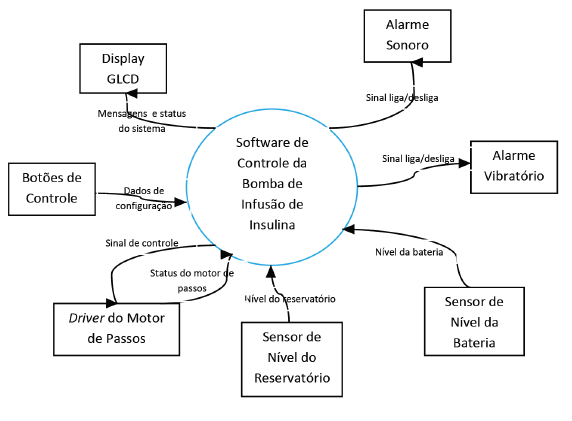
\includegraphics[scale=1]{images/contexto_bomba.png}
	\caption{Modelo de contexto da bomba de infusão de insulina}	
	\label{fig:contextobomba}
	\cite{galvao2013requirements}
\end{figure}

A divisão dos requisitos funcionas da bomba foi feita da seguinte forma:
\begin{itemize}
\item Módulo de interface com o usuário;
\item Módulo de controle de infusão;
\item Módulo de monitoramento de sensores.
\end{itemize}

Abaixo segue figuras para representar os módulos do sistema citados anteriormente. A Figura \ref{fig:usecaseinterfaceusuario} representa o móddulo de interface com o usuário, pode-se observar as possíveis ações que o usuário pode realizar de forma a interagir com o sistema. A Figura \ref{fig:usecasemoduloinfusao} representa o segundo módulo, controle de infusão, que tem a responsabilidade de administrar as duas formas de infusão: basal e bolus. O último, módulo de monitoramento dos sensores, está representado na Figuza \ref{fig:usecasemodulosensores} e é responsávels pela verificação do sistema como um todo.

\begin{figure}[htp]
	\centering
	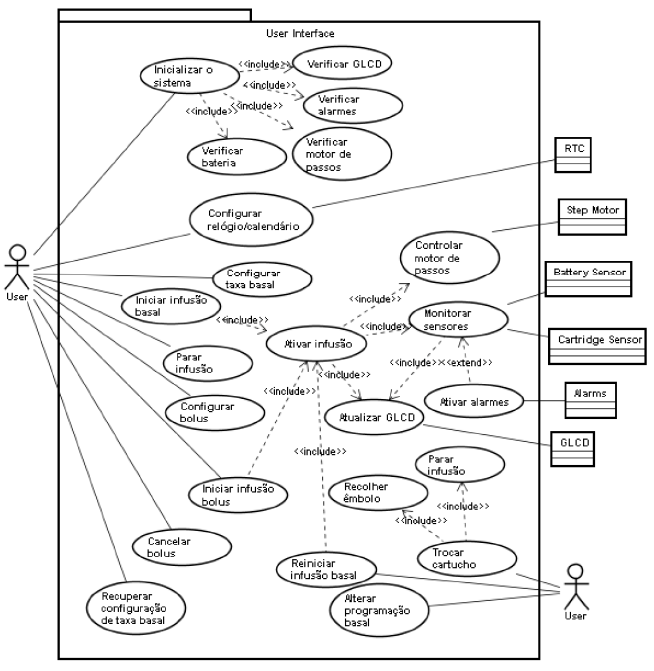
\includegraphics[scale=0.8]{images/caso_uso_interface_usuario.png}
	\caption{Caso de uso do módulo de interface com o usuário}	
	\label{fig:usecaseinterfaceusuario}
	\cite{galvao2013requirements}
\end{figure}

\begin{figure}[htp]
	\centering
	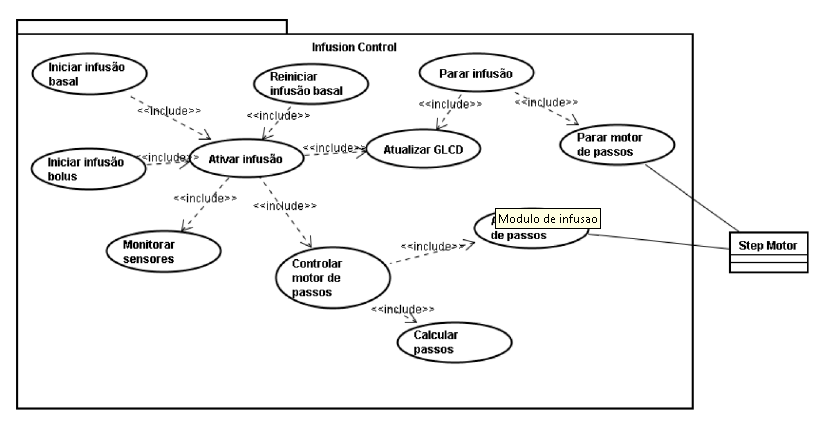
\includegraphics[scale=0.7]{images/modulo_infusao.png}
	\caption{Caso de uso do módulo de controle de infusão}	
	\label{fig:usecasemoduloinfusao}
	\cite{galvao2013requirements}
\end{figure}

\begin{figure}[htp]
	\centering
	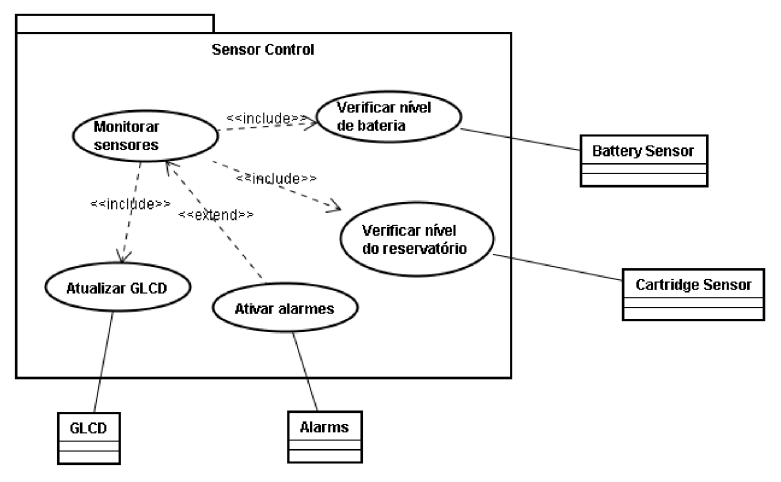
\includegraphics[scale=0.7]{images/modulo_sensores.png}
	\caption{Caso de uso do módulo de monitoramento dos sensores}	
	\label{fig:usecasemodulosensores}
	\cite{galvao2013requirements}
\end{figure}



% ----------------------------------------------------------
% Dev modulo Bomba de Infusao
% ----------------------------------------------------------
\chapter{Módulo de controle de infusão de insulina}
Este trabalho tem o objetivo de estudar e desenvolver um protótipo do módulo de controle da bomba de infusão de insulina, para o desenvolvimento vamos utilizar o microcontrolador PIC18F452. Módulo este responsável por controlar o funcionamento da bomba em função dos parâmetros recebidos e pré estabelecidos. É possível configurar a quantidade a ser infundido no período de 24 horas, infusão basal, e, além disso e mais importante, o desenvolvimento foi feito em cima do simulador proteus e devido a possibilidade de mudanças possíveis o sistema foi montado de forma que deixa os módulos desacoplados. Para isso foi utilizado o conceito OOC, \emph{Object Orientated Programming in ANSI-C}, o que possibilitou o uso de \emph{Design Patterns}.

\section{\emph{OOC - \emph{Object Orientated Programming in ANSI-C}}}
Segundo \cite{schreiner1993object}, OOC, \emph{Object Orientated Programming in ANSI-C}, é uma forma de se aproveitar as diversas vantagens da Programação orientada objeto. Vantagens essas proporcionadas por linguagens como C++, java, python, smalltalk e outras. OOC, necessita da sepação em dois arquivo distindos, separação semelhante a do c++: o primeiro possui a extensão por padrão ".h" e contém apenas a declarações de interfaces e classes, já o segundo, com extensão ".c", possui a devida implementação. Este é um conceito considerado mais denso do que Orientação Objeto propriamente dito, isso se deve ao fato de que o usuário implemente componentes como: 

\begin{itemize}
\item Interface: Define-se interface como uma \emph{struct} com ponteiros para funções, de forma que o \emph{bind} das funções é feito na hora da criação de um objeto de uma classe que implemente essa interface;
\item Classe: Da mesma forma que as interfaces, é uma \emph{struct} em que os atributos são ponteiros para função, entretanto tem os \emph{binds} definidos em uma função de criação(construtor) pertencente a essa classe, ou módulo;
\item Construtor: Função da classe em que faz o \emph{bind} de cada ponteiro para cada função da classe, alocações dinâmicas e outras operações que podem ser definidas de acordo com a necessidade de cada classe;
\item Destrutor: Basicamente a liberação de todos os recursos alocados pelo construtor e funções que a classe utilizou;
\item Public: Declaração da variável como atributo da \emph{struct} ou no arquivo \emph{header};
\item Private: Declaração da variável fora da \emph{struct}, no arquivo que tem a implementação das funções da classe.
\end{itemize}

O conceito de polimorfismo e abstração de dados se dá pela associação de um mesmo ponteiros de função de uma classe ou interface à funções diferente, variando em função da classe mais especializada que está sendo abstraída.

Obviamente é uma simulação da consolidada programação orientada objeto e possui limitações como: Programação genérica sem validação em tempo de compilação, sintaxe mais complexa, geração de código implícito, entre outros. Entretanto ainda permite reutilização de código e, como dito anteriormente, abstração de dados.

\section{\emph{Design Patterns}}
Na engenharia de \emph{software}, um \emph{Design Patterns} ou padrão de projeto é uma solução repetível geral para um problema comumente ocorre em \emph{design} de \emph{software}. Um padrão de projeto não é um projeto acabado que pode ser transformado diretamente em código. É uma descrição ou modelo de como resolver um problema que pode ser utilizado em diversas situações diferentes. \cite{shalloway2004design}.

\subsection{Usos de \emph{Design Patterns}}

Os \emph{Design Patterns} podem acelerar o processo de desenvolvimento, fornecendo testados e comprovados paradigmas de desenvolvimento. O \emph{design} de \emph{software} eficaz requer considerar as questões que não podem tornar-se visível até mais tarde na implementação. Reutilizar \emph{Design Patterns} ajuda a prevenir situações que podem causar grandes problemas e melhora a legibilidade do código para programadores e arquitetos familiarizados com os padrões.

Muitas vezes, as pessoas só entendem como aplicar certas técnicas de \emph{design} de \emph{software} para determinados problemas. Estas técnicas são difíceis de aplicar a uma ampla gama de problemas. Os \emph{Design Patterns} fornecem soluções gerais, documentadas em um formato que não requer especificidades ligadas a um problema particular \cite{shalloway2004design}.

Segundo \cite{shalloway2004design}, além disso, os padrões permitem que os desenvolvedores se comuniquem usando nomes bem conhecidos e bem compreendidos para interações de software. \emph{Design Patterns} comuns podem ser melhorados ao longo do tempo, tornando-os mais robustos do que os projetos ad-hoc, ou seja, problemas específicos. Os \emph{Design Patterns} podem ser divididos em:

\begin{itemize}
\item \emph{Creational design patterns}: Estes \emph{Design Patterns} tem tudo a ver com padrões de instanciação de classe. Esse padrão pode ser dividido em padrões de criação de classe e de criação de objetos. Enquanto os padrões de criação de classe usam a herança de forma eficaz no processo de instanciação, os padrões de criação de objeto usam a delegação de forma eficaz para ter o trabalho de criação feito. 
\item \emph{Structural design patterns}: Este \emph{Design Pattern} tem tudo a ver com composição de classe e objetos. Padrão estrutural de classe usa a herança para compor interfaces. Padrão estrutural de objeto define formas de compor objetos para obter novas funcionalidades.
\item \emph{Behavioral design patterns}: São os padrões que são mais especificamente relacionadas com a comunicação entre objetos.
\end{itemize}

\subsection{\emph{Factory Method}}
Segundo \cite{shalloway2004design}, \emph{factory method} foi um dos \emph{Design Patterns} escolhidos para esse projeto. Seus objetivos principais são:

\begin{itemize}
\item Definir uma interface para criar um objeto, mas deixa as subclasses decidirem qual classe instanciar. Factory Method permite adiar a instanciação da classe para a subclasses;
\item Definir um construtor \emph{virtual};
\item Operador \emph{new} é considerado perigoso.
\end{itemize}

Esse \emph{Design Patterns} foi utilizado no módulo que faz uso do \emph{display} de LCD para que a troca de seu tipo ficasse isolado do restante do sistema e que um futura troca possa ser feita com o menor impacto possível. A Figura \ref{fig:factorymethod} representa sua etsrutura em UML. \newpage

\begin{figure}[htp]
	\centering
	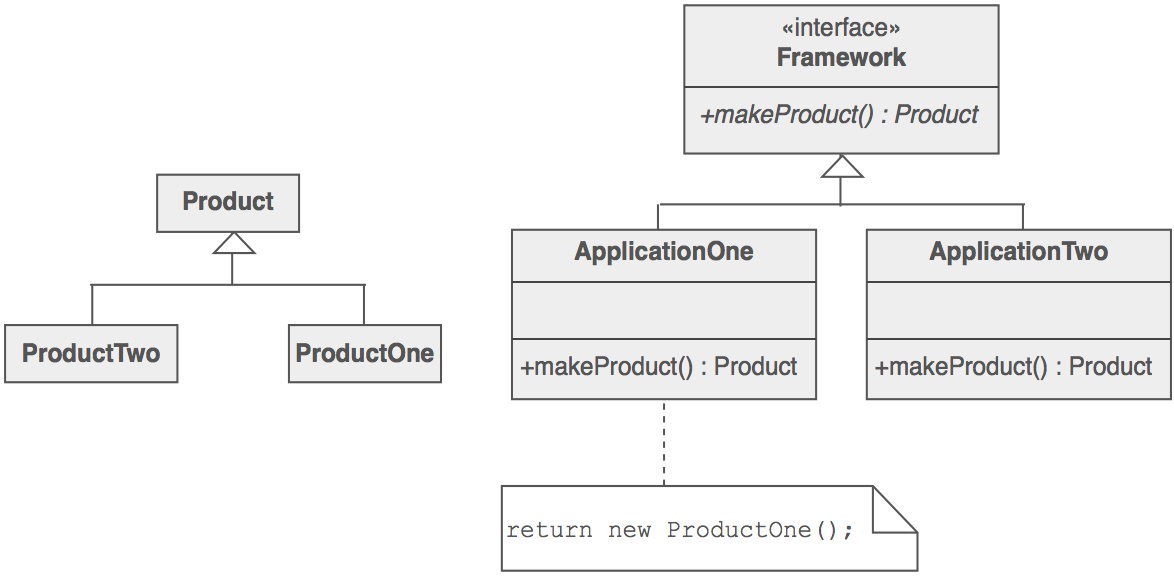
\includegraphics[scale=0.4]{images/Factory_Method.png}
	\caption{Estrutura do padrão \emph{Factory Method}}	
	\label{fig:factorymethod}
	\cite{shalloway2004design}
\end{figure}

\section{Proteus}

No desenvolvimento deste TCC o simulador Proteus foi usado para montar o ambiente de tesste. Para testes, o circuito teve seu desenvolvimento em função dos seguintes componentes: microcontrolador da família PIC, PIC18F452, motor de passo, \emph{display} de LCD 2x16, botões e driver para o motor de passo. A Figura \ref{fig:proteus} representa a imagem do \emph{Software}.

\begin{figure}[htp]
	\centering
	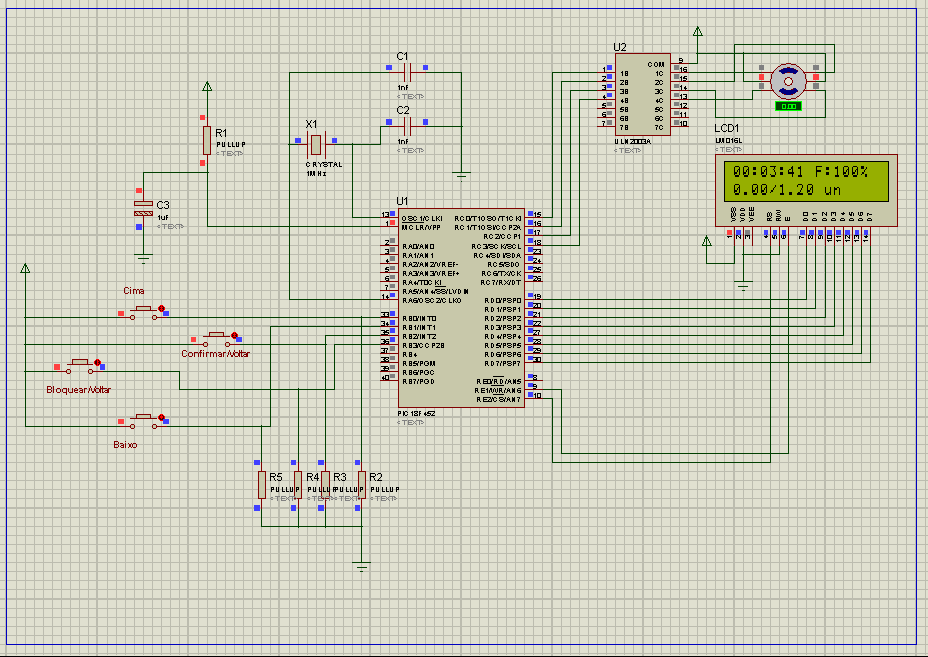
\includegraphics[scale=0.5]{images/proteus.png}
	\caption{\emph{Software} Proteus}	
	\label{fig:proteus}
\end{figure}

\section{Arquitetura do Software}

O \emph{Software} foi desenvolvido de forma modular para que as funções fossem facilmente testadas, modificadas e evoluídas, a Figura \ref{fig:arquiteturageral} representa a estrutura citada. A divisão do \emph{Software} foi feita da seguinte forma: config, insulimpump, lcd, menu, motor, timerMotor e principal. 

\begin{figure}[htp]
	\centering
	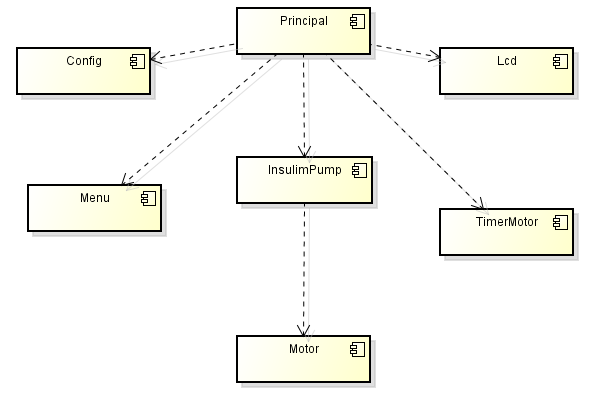
\includegraphics[scale=0.7]{images/arquitetura.png}
	\caption{Estrutura do \emph{Software}}	
	\label{fig:arquiteturageral}
\end{figure}

\subsection{Módulo Config}

Módulo feito para centralizar todas as configurações do sistema, utilizado, basicamente, por quase todos os demais módulos. Seguindo parte do conceito de OOC, pois foi possível utilizar a ideia de \emph{private} e \emph{public} para as variáveis. Entretanto não foi criada nenhuma \emph{struct} de forma que representasse uma classe. A Figura \ref{fig:driagramaclasseconfig} representa o diagrama de classe desse módulo. \newpage


\begin{figure}[htp]
	\centering
	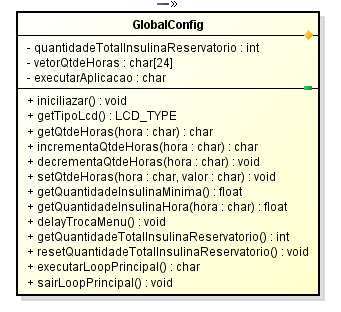
\includegraphics[scale=1]{images/classe_GlobalConfig.png}
	\caption{Diagrama de classe GlobalConfig}	
	\label{fig:driagramaclasseconfig}
\end{figure}

Quando se diz \emph{private} e \emph{public} é o fato de adicionar as variáveis no arquivo GlobalConfig.h, \emph{private}, ou GlobalConfig.c, \emph{public}. A principal parametrização desse módulo é a quantidade que o repositório de insulina suporta. Para modificar seu valor basta alterar o \emph{define} QUANTIDADE\_TOTAL\_RESERVATORIO\_INSULINA. Esse valor representa a quantidade de insulina existente no reservatório na escala da infusão mínima da bomba.

\subsection{Módulo InsulinPump}

O módulo InsulinPump é responsável pela abstração das funções da bomba para o resto do sistema. Funções simples para o resto do sistema como: inicializar variáveis de controle, iniciar operação, parar operação - principalmente para configurações da bomba -, injetar e retornar a quantidade inserida naquela hora. Seguindo o conceito OOC foi criada uma "interface", IInsulinPump, e a "classe" concreta InsulinPump. A Figura \ref{fig:diagramainsulinpump} representa a relação e diagrama de classe dos elementos citados anteriormente.

\begin{figure}[htp]
	\centering
	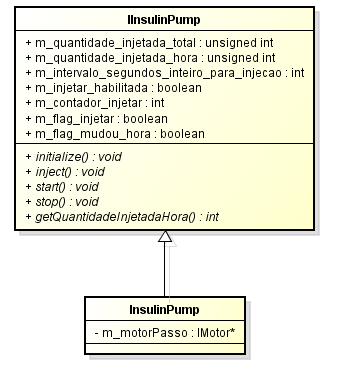
\includegraphics[scale=1]{images/classe_insulinpump.png}
	\caption{Diagrama de classe InsulinPump}	
	\label{fig:diagramainsulinpump}
\end{figure}

\subsection{Módulo Lcd}

Esse módulo é responsável pelo isolamento do \emph{display} de LCD do resto do sistema. Composto por um \emph{factory}, que retorna um obeto de controle de acordo com o parâmetro passado, uma "interface" para possibilitar essa abstração e as classes concretas, no caso existe apenas a classe concreta para \emph{display} 2x16(2 linhas por 16 colunas). A Figura \ref{fig:diagramalcd} representa a relação e diagrama de classe dos elementos citados anteriormente.

\begin{figure}[htp]
	\centering
	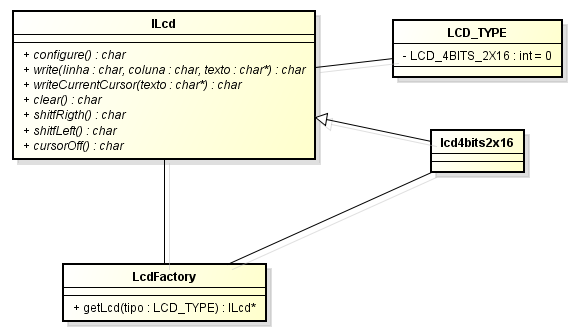
\includegraphics[scale=0.8]{images/classe_lcd.png}
	\caption{Diagrama de classe Lcd}	
	\label{fig:diagramalcd}
\end{figure}

\subsection{Módulo Menu}

O módulo de menu foi criado para abstrair todos as possíveis situações e estados da bomba. Foi criado de uma forma muito simples e é equivalente a uma máquina de estado. Utiliza uma "inteface" que é implementado por todos os tipos de menu existentes como: menu de confuguração da bomba, menu da bomba em execução, menu de confirmação do estado do reservatório e outros. A Figura \ref{fig:classemenu} representa as relações entre os componentes, ou "classes", do módulo e demonstra como é simples a criação de novos menus.

\begin{figure}[htp]
	\centering
	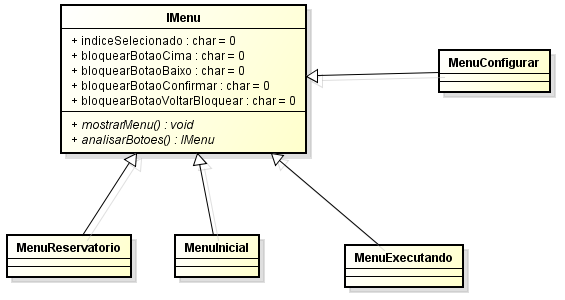
\includegraphics[scale=1]{images/classe_menu.png}
	\caption{Diagrama de classe Menu}	
	\label{fig:classemenu}
\end{figure}

\subsection{Módulo Motor}

O módulo motor, tem como resposabilidade abstrair todas as operações necessárias para o controle do motor de forma que o resto do sistema não saiba qual motor está utilizando. Isso é possível devido a "interface" criada para abstração e o uso de um \emph{Factory} que retorna o motor que deve ser utilizado de acordo com um parâmetro global, localizado no módulo config. A figura \ref{fig:classemotor} representa as relações existentes nesse módulo. \newpage


\begin{figure}[htp]
	\centering
	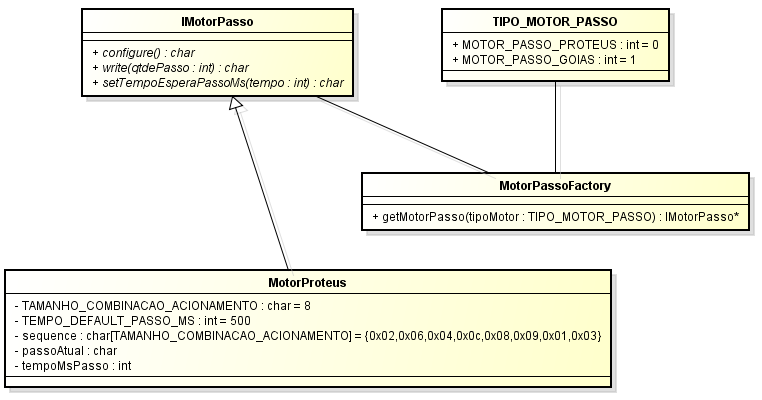
\includegraphics[scale=0.8]{images/classe_motor.png}
	\caption{Diagrama de classe Motor}	
	\label{fig:classemotor}
\end{figure}

\subsection{Módulo TimerMotor}

O módulo TimerMotor armazena todos os dados do contador para o uso dos motores. Abstrai a configuração do timer em função do \emph{hardware} para o resto do sistema. Dessa forma o sistema só precisa se preocupar em: fazer configuração inicial(inicializar variáveis), iniciar timer, parar timer. A Figura \ref{fig:classe_timer_motor} representa a relação citada acima.

\begin{figure}[htp]
	\centering
	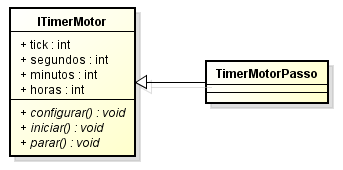
\includegraphics[scale=1]{images/classe_timer_motor.png}
	\caption{Diagrama de classe TimerMotoror}	
	\label{fig:classe_timer_motor}
\end{figure}


\subsection{Módulo Principal}

Devido a forma modular com  que foi implementado o sistema esse tornou-se o módulo mais simples. Ficou responsável apenas pela interrupção, específico do hardware, chamar os métodos de incialização dos módulos do lcd, TimerMotor e InsulinPump, e um loop principal, extremamente simples, que exibe o Menu, correspondente ao estado atual, e recebe o retorno do próprio menu em questão para navegar entre os menus existente.

\chapter{Análise e discussão dos resultados}

\section{Simulador}

O uso do simulador foi importantíssimo para o desenvolvimento desse trabalho. Ele possibilitou iniciar o desenvolvimento sem uma placa física. Utilizando-o montou-se um circuito exemplo utilizando o microcontrolador escolhido e, de forma iterativa, era possível evoluir tanto o circuito quanto o software, por exemplo: montou-se o circuito com o LCD e implementou-se o módulo de controle do mesmo, adicionou-se os componentes de menu e a análise de botões, e outros passos. Vendo esses passos é possível perceber que o desenvolvimento foi feito por funcionalidade isoladas de forma que fosse possível testar cada "parte" do software e assim minimizar os problemas do \emph{software} como um todo e assim sempre ter um versão estável, mesmo que mínima.

Além de todas essas facilidades, a gama de testes e depuração é maior em um simulador do que no \emph{hardware}, como: o simulador indica más práticas existentes, permite simular o uso da bomba por dias em questão de minutos, basta configurar o tempo de execução, e outros. Graças aos exemplos citados anteriormente foi possível encontrar diversos problemas que só seriam descobertos quando estivesse testando diretamente no \emph{hardware} e mesmo assim surgiria a dúvida: É o \emph{hardware} ou o \emph{software}.

O circuito elétrico utilizado para os testes foi desenvolvido com base na placa Microgenios, representada pela Figura \ref{fig:microgenios}. Todos os componentes utilizados assim como as ligações entre eles são fiéis à placa de referência, salvo às ligações do motor que não faz parte do conjunto de referência. Portanto uma migração para a placa de Microgenios teria o funcionamento dos botões existentes e \emph{display} de LCD de acordo com o esperado.

E, além disso, como os testes e validações do \emph{hardware} feito através simulador são extremamente válidas e consistentes e o desenvolvimento foi baseado em uma placa consolidada, uma integração com uma placa diferente da utilizada como referência será muito mais simples. Isso deve-se ao fato através do simulador diminui-se os riscos e problemas no período de integração, onde são encontrados as maiores e inesperadas dificuldades do desenvolvimento.
 
 \newpage
 
 \begin{figure}[htp]
 	\centering
 	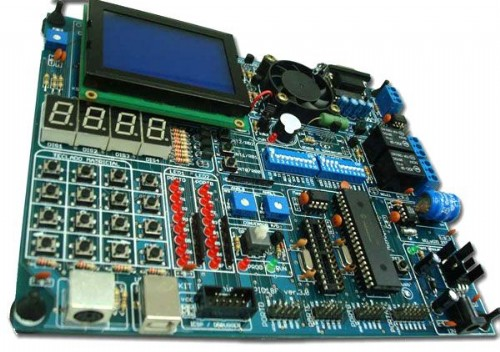
\includegraphics[scale=1]{images/pic_microgenio.png}
 	\caption{Placa Microgenios PIC18F4452}	
 	\label{fig:microgenios}
 	\cite{galvao2013requirements}
 \end{figure}

\section{Arquitetura modularizada}

A forma com que foi organizado o código é a grande vantagem desse trabalho. O desacoplamento foi o foco principal durante todo o desenvolvimento isso para facilitar mudanças no próprio \emph{software} ou mudança do \emph{hardware}

OOC foi o conceito utilizado para que fosse possível fazer testes, mocks no sistema, pelo fato de simular programação orientação à objetos. Devido a forma com que foi implementado, foi possível realizar testes utilizando um PC. O ambiente utilizado: Ubuntu 13.10, compilador gcc, Framework C++ Qt e IDE QtCreator. Como o conceito de OOC é baseado em ponteiros de função o mock das funções foi feito apenas apontando para uma função que foi criada de acordo com a situação de teste desejada. Quanto o acesso aos periféricos, todos os acionamentos e comunicações foram redirecionadas para um arquivo log de acompanhamento. A seguir será descrito as vantagens principais de cada módulo devido a forma de implementação.

O módulo Config é o mais simples de todos, Sua principal vantagem é o fato de centralizar todas as informações de configuração, fazendo com que o sistema fique mais claro. Além disso, criar casos de testes torna-se simples, pois mudando qualquer uma de suas informações já se reflete no sistema com um todo. É importante lembrar também que ele não carrega nenhuma dependência do compilador ou do hardware, foi implementado em ANSI-C, o que permite que seja utilizado por qualquer compilador e \emph{hardware}.

Os demais módulos foram criados para seguir a ideia de isolação do módulo config. Para isso o que foi feito é deixar as interfaces e funções comuns independente de \emph{hardware} e compilador utilizando apenas ANSI-C. Dessa forma, caso precise de alguma mudança mais drástica relacionada aos dois itens citados o impacto seja mínimo, precisando fazer apenas um de-para das funcionalidades específicas. 

Tendo dito as vantagens com relação à mudanças \emph{hardware} e compilador é importante lembrar que a expansibilidade e manutenibilidade do software ficou incrivelmente simples. A ideia foi deixar o "motor" ou "coração" da bomba ter conhecimento apenas das "interface" do sistemas. Dessa forma os detalhes de funcionamento, requisitos de segurança, configurações específicas de hardware para controle dos periféricos e outros, podem ser modificadas sem impactar o funcionamento básico da bomba de infusão. O mais importante é que essas alterações são parametrizável,se localizam no módulo config, e o software sabe quais objetos utilizar e de onde recuperá-los, em algum \emph{Factory} na maioria dos casos. Devido a isso tudo é possível manter mais de um produto em um único código e mudanças importantes no \emph{core} do sistema não precisa ser replicadas e correr risco de conflito entre projetos. Graças ao uso do OOC para criar algo novo basta implementar as funções da interface do módulo em questão e adicionar ao \emph{factory}, caso exista. Segue uma breve explicação do que pode ser feito em cada módulo.

O módulo InsulinPump, responsável por abstrair particularidades de funcionalidades e segurança do bomba para o resto do ambiente permite que se crie vários tipos de bomba. Essa criação leva em conta mudanças nos dois itens citados, por exemplo, bomba europeia, americana, brasileira, que podem ter requisitos de segurança distintos.

O módulo LCD, responsável por abstrair a forma de uso e qual \emph{display} está sendo utilizado. Ele permite a troca do tipo de LCD utilizado seja simples, por exemplo, trocar o utiliza 2x16, por um 2x12.

O módulo Menu, lembra uma máquina de estado retorna um próximo Menu(estado) ou ele mesmo caso a mudança não ocorra. Para adicionar um novo menu é só adicionar como retorno em alguma situação dentro da função de análise de botões que todos os Menus possuem.

O módulo Motor segue a mesma linha do LCD, permite a troca do periférico por outro motor de passo ou até mesmo um outro tipo de motor.

O módulo TimerMotor foi criado para desvincular o \emph{timer} que é extremamente dependente do \emph{hardware} e compilador. Foi o módulo mais complicado de se isolar e é o único que não está totalmente isolado devido a algumas limitações do execução de interrupções.
% ---
% Finaliza a parte no bookmark do PDF, para que se inicie o bookmark na raiz
% ---
\bookmarksetup{startatroot}% 
% ---

% ---
% Conclusão
% ---
\chapter{Conclusão}

Este trabalho teve como base o desenvolvimento de um sistema embarcado para controle de infusão de um protótipo de uma bomba de infusão de insulina, além de comunicação com periféricos para interação com o usuário. O módulo desenvolvido é responsável por executar os perfis de infusão configurados pelo o usuário, ativar o motor de passos, dar \emph{feedback} do status da bomba e de sua execução ao paciente. Os objetivos desse trabalho foram alcançados ao desenvolver o módulo de controle, utilizando o microcontrolador PIC de baixo custo: PIC18F452. 

A compreensão das tecnologias utilizadas, simulador e, é claro, da natureza do problema proposto foram imprescindíveis. O presente trabalho pode ser considerado uma prova de conceito do módulo desenvolvido, e pode ser continuado e aprimorado sem grandes problemas devido a sua alta modularidade e simplicidade do código. E com isso realizar testes mais precisos e factíveis com relação a realidade do problema proposto. 

Considerando como projeto futuro seria os testes utilizando um \emph{hardware}, placa da Microgenios citada anteriormente, composto pelos componentes abordados e comprovar as vantagens do uso do simulador, demonstrar que testes de \emph{stress}, ou seja, por longos períodos pode sem simulado no PC, graças ao OOC. E, por fim, talvez menos importante, conseguir isolar completamente a dependência do compilador e \emph{hardware} devido à forma de uso da interrupção para contagem de tempo para infusão.

Por fim, o código é aberto e pode ser encontrado em: \url{https://gitlab.com/dinesh/insulin_pump}.


% ----------------------------------------------------------
% ELEMENTOS PÓS-TEXTUAIS
% ----------------------------------------------------------
\postextual


% ----------------------------------------------------------
% Referências bibliográficas
% ----------------------------------------------------------
%\bibliographystyle{plain}
\bibliography{references}

% ----------------------------------------------------------
% Glossário
% ----------------------------------------------------------
%
% Consulte o manual da classe abntex2 para orientações sobre o glossário.
%
%\glossary

% ----------------------------------------------------------
% Apêndices
% ----------------------------------------------------------

% ---
% Inicia os apêndices
% ---
\begin{apendicesenv}


% Imprime uma página indicando o início dos apêndices
\partapendices

% ----------------------------------------------------------
\chapter{Config}
% ----------------------------------------------------------

\section{Config.c}

\lstinputlisting[language=C]{../../insulin_pump/src/config/GlobalConfig.c}
	
\section{Config.h}

\lstinputlisting[language=C]{../../insulin_pump/src/config/GlobalConfig.h}




% ----------------------------------------------------------
\chapter{InsulinPump}
% ----------------------------------------------------------

\section{IInsulinPump.h}

\lstinputlisting[language=C]{../../insulin_pump/src/InsulinPump/IInsulinPump.h}

\section{InsulinPump.c}

\lstinputlisting[language=C]{../../insulin_pump/src/InsulinPump/InsulinPump.c}
	
	
\section{InsulinPump.h}

\lstinputlisting[language=C]{../../insulin_pump/src/InsulinPump/InsulinPump.h}
	

% ----------------------------------------------------------
\chapter{Lcd}
% ----------------------------------------------------------

\section{lcd.h}

\lstinputlisting[language=C]{../../insulin_pump/src/lcd/lcd.h}
	
\section{lcdFactory.h}

\lstinputlisting[language=C]{../../insulin_pump/src/lcd/lcdFactory.h}

\section{lcdFactory.c}

\lstinputlisting[language=C]{../../insulin_pump/src/lcd/lcdFactory.c}


\section{lcd4bits2x16}

\subsection{lcd4bits2x16.h}

\lstinputlisting[language=C]{../../insulin_pump/src/lcd/lcd4bits2x16/lcd4bits2x16.h}

\subsection{lcd4bits2x16.c}

\lstinputlisting[language=C]{../../insulin_pump/src/lcd/lcd4bits2x16/lcd4bits2x16.c}


% ----------------------------------------------------------
\chapter{Menu}
% ----------------------------------------------------------

\section{IMenu.h}

\lstinputlisting[language=C]{../../insulin_pump/src/menu/IMenu.h}
	
\section{MenuConfigurar.h}

\lstinputlisting[language=C]{../../insulin_pump/src/menu/MenuConfigurar.h}

\section{MenuConfigurar.c}

\lstinputlisting[language=C]{../../insulin_pump/src/menu/MenuConfigurar.c}


\section{MenuExecutando.h}

\lstinputlisting[language=C]{../../insulin_pump/src/menu/MenuExecutando.h}

\section{MenuExecutando.c}

\lstinputlisting[language=C]{../../insulin_pump/src/menu/MenuExecutando.c}


\section{MenuInicial.h}

\lstinputlisting[language=C]{../../insulin_pump/src/menu/MenuInicial.h}

\section{MenuInicial.c}

\lstinputlisting[language=C]{../../insulin_pump/src/menu/MenuInicial.c}


\section{MenuReservatorio.h}

\lstinputlisting[language=C]{../../insulin_pump/src/menu/MenuReservatorio.h}

\section{MenuReservatorio.c}

\lstinputlisting[language=C]{../../insulin_pump/src/menu/MenuReservatorio.c}

% ----------------------------------------------------------
\chapter{Motor}
% ----------------------------------------------------------

\section{IMotorPasso.h}

\lstinputlisting[language=C]{../../insulin_pump/src/motor/IMotorPasso.h}
	
\section{MotorPassoFactory.h}

\lstinputlisting[language=C]{../../insulin_pump/src/motor/MotorPassoFactory.h}

\section{MotorPassoFactory.c}

\lstinputlisting[language=C]{../../insulin_pump/src/motor/MotorPassoFactory.c}


\section{MotorProteus}

\subsection{MotorProteus.h}

\lstinputlisting[language=C]{../../insulin_pump/src/motor/MotorProteus/MotorProteus.h}

\subsection{MotorProteus.c}

\lstinputlisting[language=C, breaklines=true]{../../insulin_pump/src/motor/MotorProteus/MotorProteus.c}


% ----------------------------------------------------------
\chapter{TimerMotor}
% ----------------------------------------------------------

\section{ITimerMotor.h}

\lstinputlisting[language=C]{../../insulin_pump/src/timerMotor/ITimerMotor.h}
	
\section{TimerMotorPasso.h}

\lstinputlisting[language=C]{../../insulin_pump/src/timerMotor/TimerMotorPasso.h}

\section{TimerMotorPasso.c}

\lstinputlisting[language=C]{../../insulin_pump/src/timerMotor/TimerMotorPasso.c}

% ----------------------------------------------------------
\chapter{Principal}
% ----------------------------------------------------------

\section{insulin\_pump.c}

\lstinputlisting[language=C, breaklines=true]{../../insulin_pump/insulin_pump.c}


\end{apendicesenv}

\end{document}
